\section{Experiments and Results}\label{sec:exp_and_results}

\subsection{Synthetic Data}\label{sec:synthetic}

\asubsubsection{\texttt{AbsoluteLayer} -- Unlabeled}{Tomáš Sláma}

\textit{The results are taken from the \href{https://github.com/xiaoxiae/GNNFinal2024/blob/main/notebooks/abs.ipynb}{notebooks/abs.ipynb} notebook.}

The initial experiment was to compare performance on the four datasets the original paper used with the following baseline network architecture (NF). The sizes of the layers were chosen to sufficiently capture the complexity of all of the datasets:


\begin{minted}{python}
(BijectiveLayer(2, [64] * 5), OrthonormalLayer(2)) x 10
\end{minted}

To utilize the symmetry of the data, this architecture was compared with one that has an absolute layer at the beginning (NF-abs):

\begin{minted}{python}
AbsoluteLayer(2)
(BijectiveLayer(2, [64] * 5), OrthonormalLayer(2)) x 10
\end{minted}

The results can be seen in figure \ref{fig:abs-default}. Unless specified otherwise, all networks in this section were trained for $1\,000$ epochs with a learning rate $0.001$ and batch size $1\,000$.

\begin{figure}[H]
    \centering
    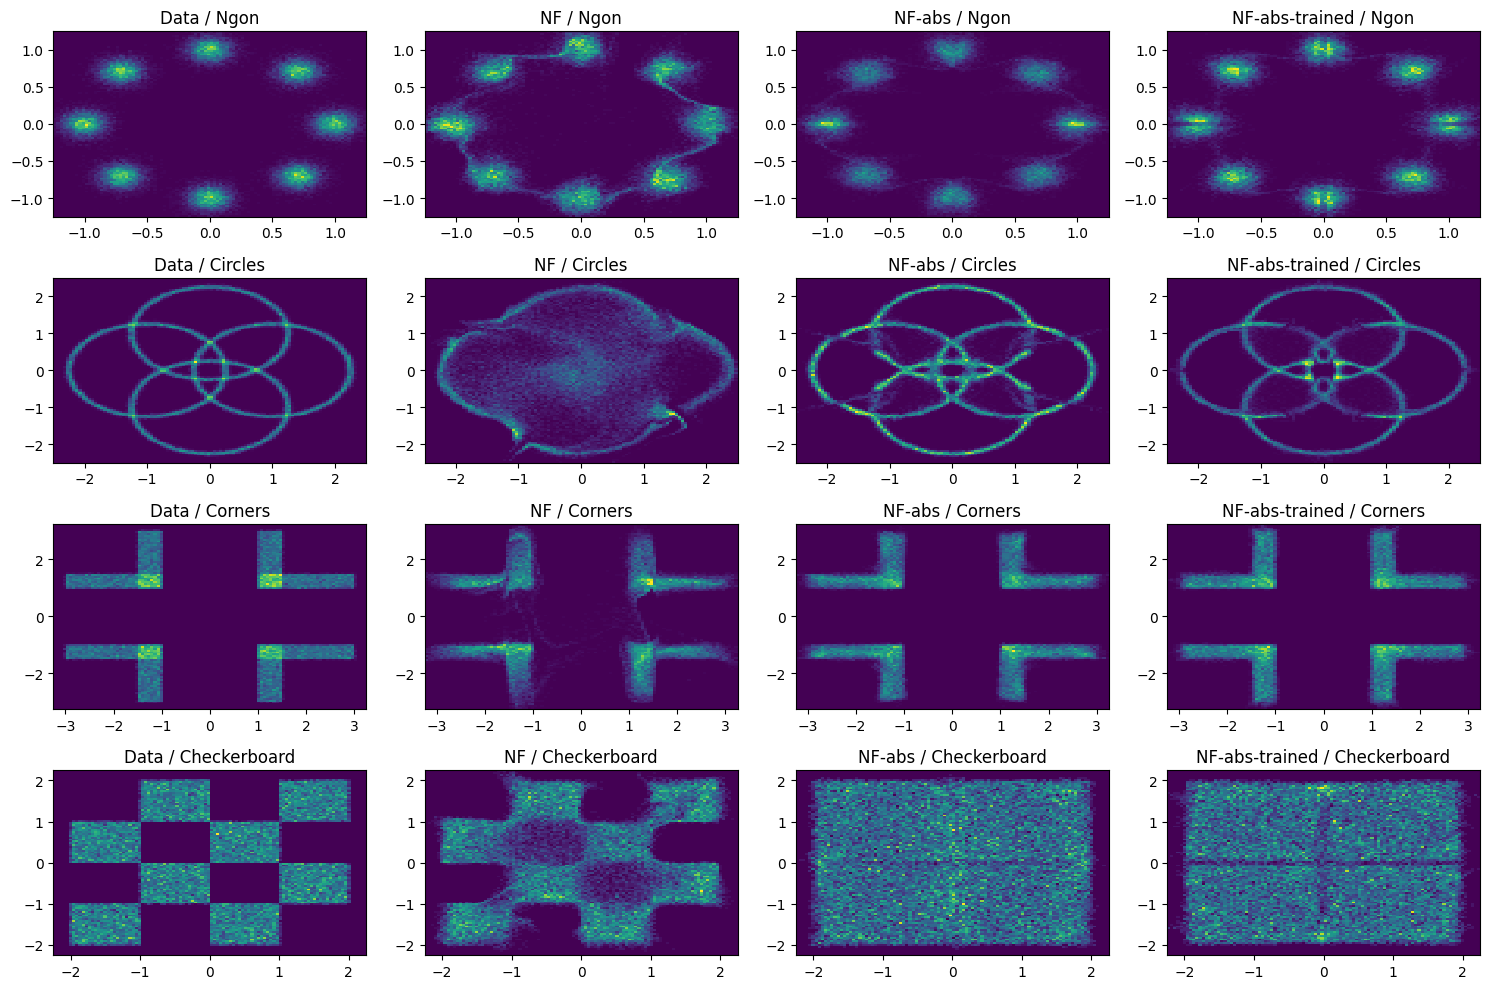
\includegraphics[width=.85\linewidth]{images/synthetic/abs-default.png}
    \caption{Comparison of methods for synthetic datasets; ground truth (column 1), baseline network architecture (column 2), architecture with absolute layer at the beginning with a fixed Q-tensor (column 3) and architecture with absolute layer at the beginning with a learned Q-tensor (column 4).}
    \label{fig:abs-default}
\end{figure}

As we see, the architectures with the absolute layer (columns 3 and 4) perform much better, which is no surprise since it dictates the symmetry in both axes and is therefore much easier to train.

As a sanity check, the models were also trained on skewed data (i.e. $50\%$ of values were randomly flipped about the Y-axis) to see if the absolute layer learned the correct Q-tensor. The result can be seen in Figure \ref{fig:abs-skewed}.

\begin{figure}[H]
    \centering
    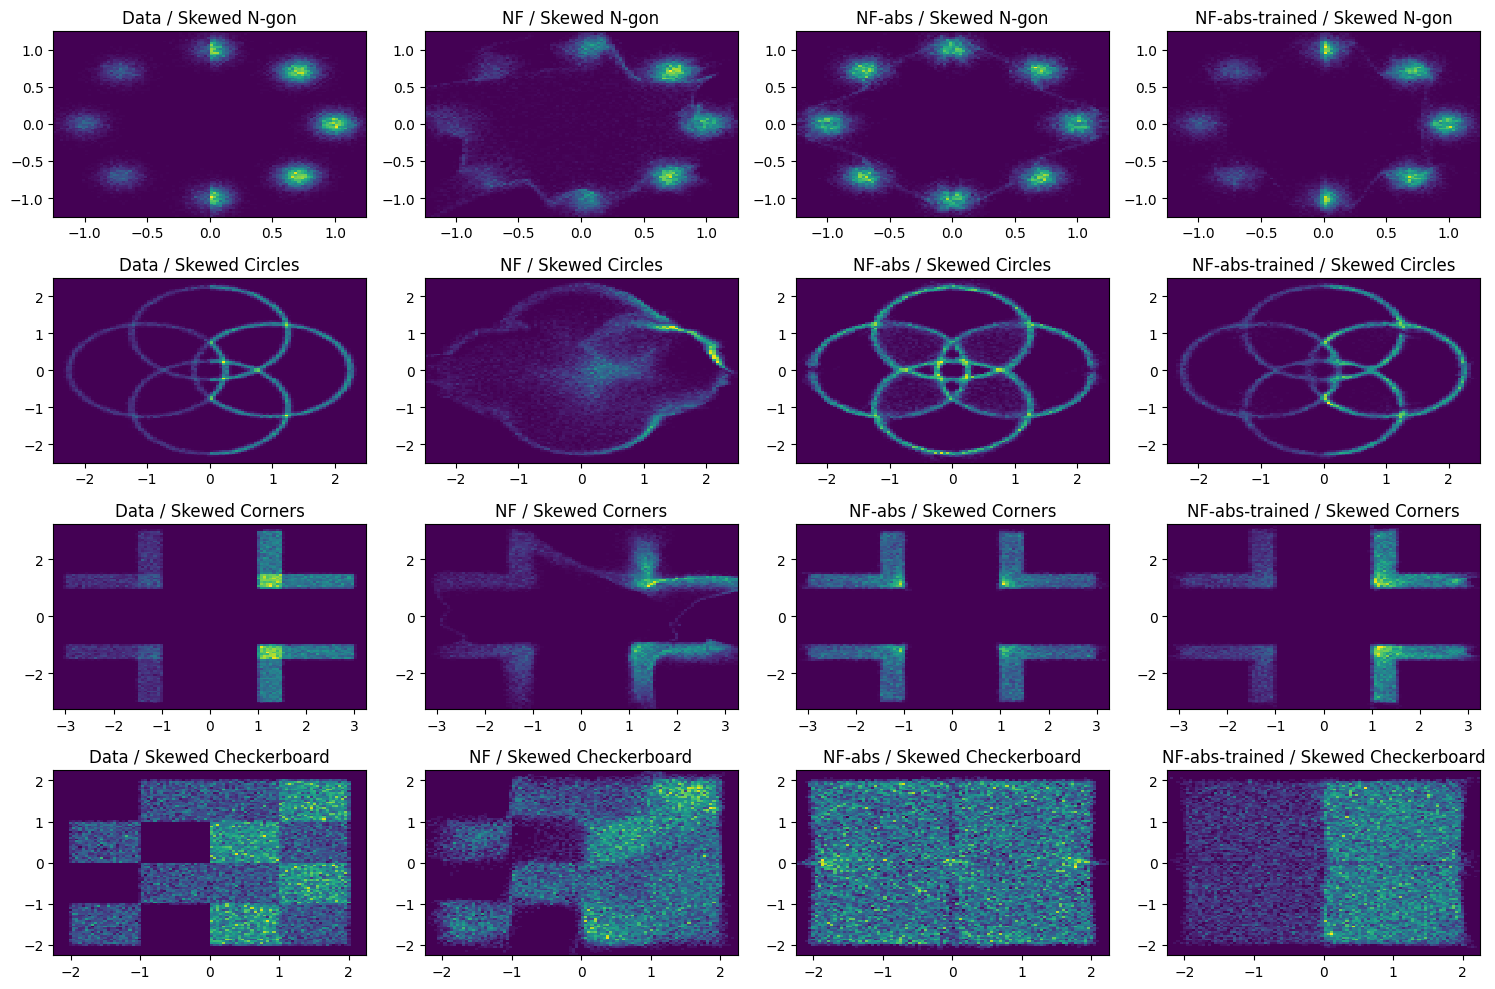
\includegraphics[width=.85\linewidth]{images/synthetic/abs-skewed.png}
    \caption{Comparison of methods for \textit{skewed} synthetic datasets; columns are same as Figure \ref{fig:abs-default}.}
    \label{fig:abs-skewed}
\end{figure}

\begin{figure}[H]
    \centering
    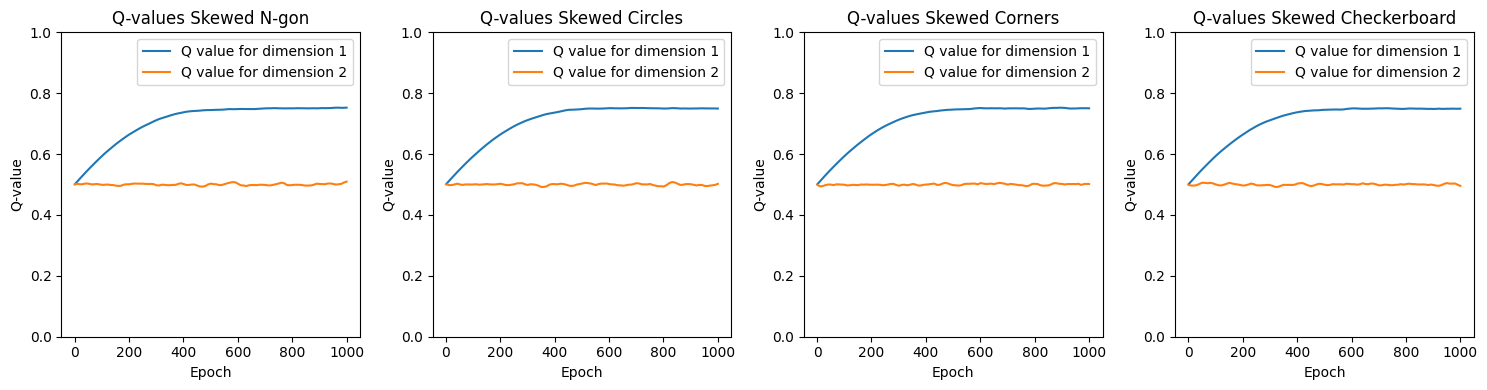
\includegraphics[width=.85\linewidth]{images/synthetic/skewed-q.png}
    \caption{Q-values for the last model of Figure \ref{fig:abs-skewed}.}
    \label{fig:skewed-q}
\end{figure}

The network indeed learns the correct Q-values of $0.75$ (since we flipped half of the data, i.e. the split becomes 25\%/75\%) for the $x$-axis, while the $y$-axis stays at $0.5$ (since it wasn't skewed).

Since this works well for a centered normalized dataset, the next step is to offset it by a constant (so the axes of symmetry are no longer the origin).  
The results can be seen in Figure \ref{fig:abs-offset}.

\begin{figure}[p]
    \centering
    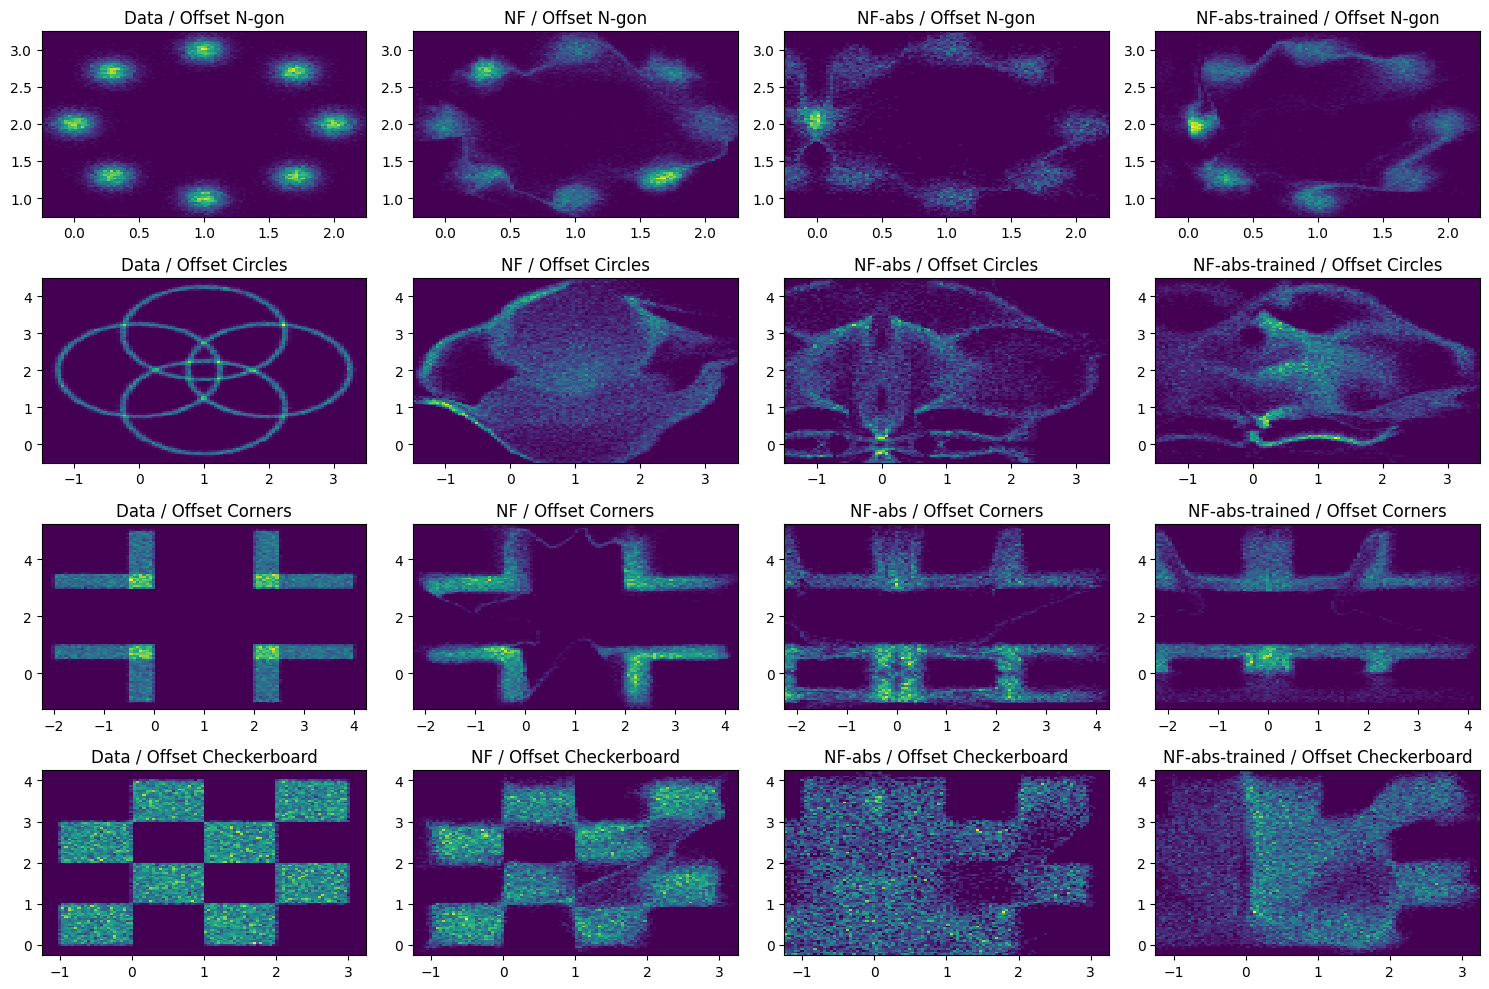
\includegraphics[width=.85\linewidth]{images/synthetic/abs-offset.png}
    \caption{Comparison of methods for \textit{offset} synthetic datasets; columns are same as Figure \ref{fig:abs-default}.}
    \label{fig:abs-offset}
\end{figure}

\begin{figure}[p]
    \centering
    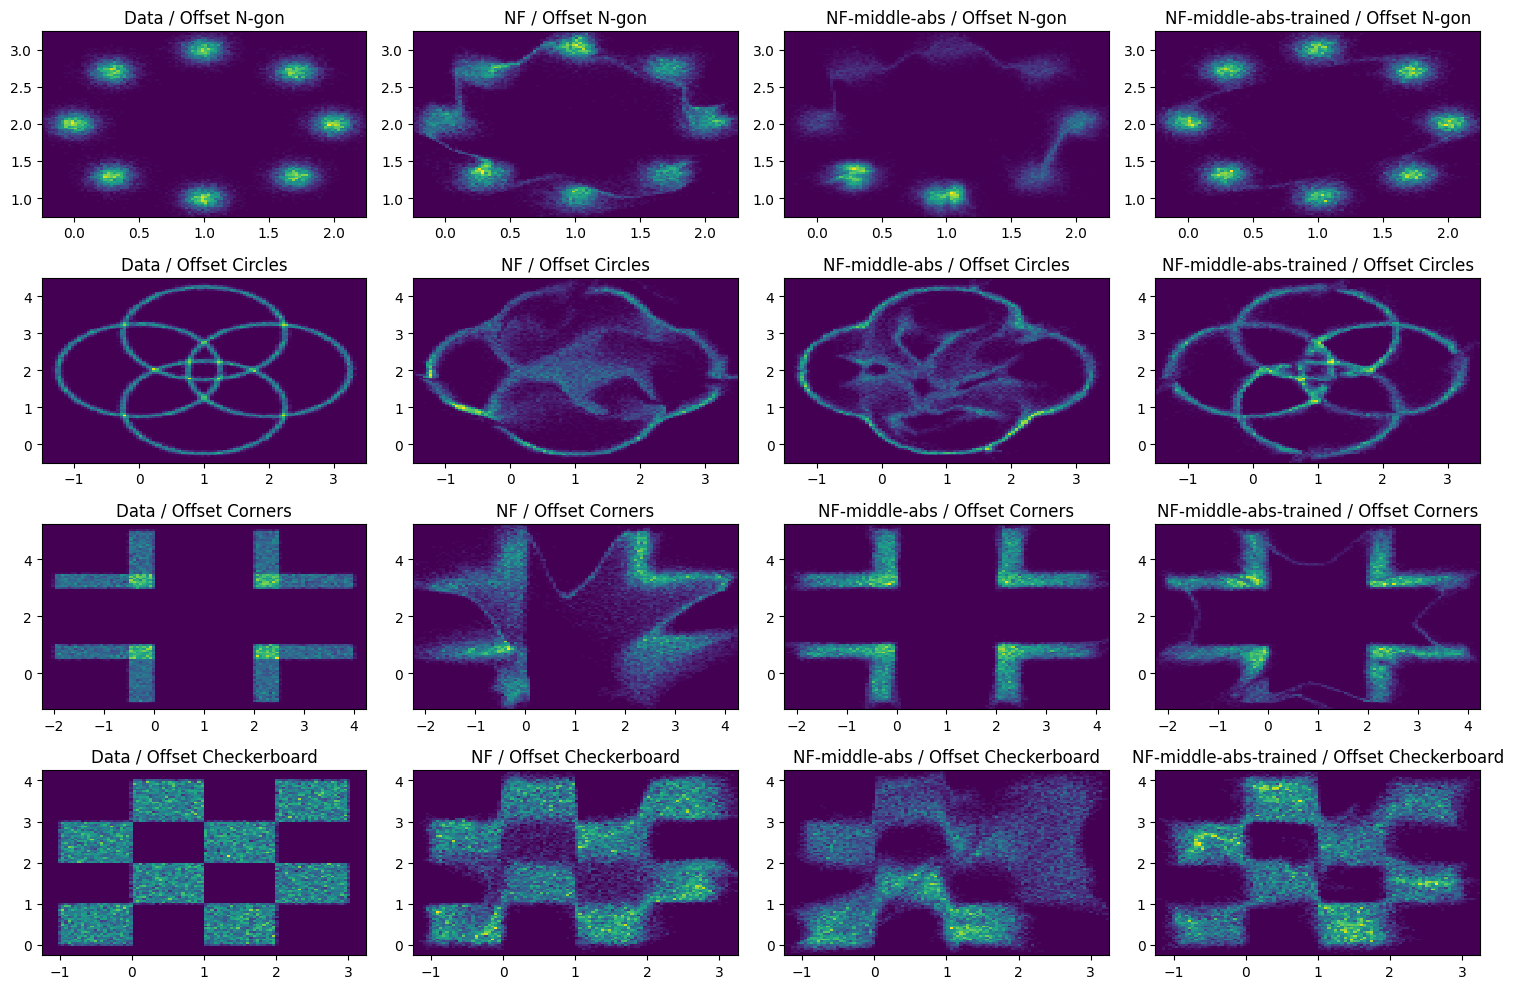
\includegraphics[width=.85\linewidth]{images/synthetic/abs-offset-fixed.png}
    \caption{Comparison of methods for \textit{offset} synthetic datasets; first two columns are same as Figure \ref{fig:abs-default}, last two are changed by moving the absolute layer in the middle.}
    \label{fig:abs-offset-fixed}
\end{figure}

Unsurprisingly, this breaks the architectures with an absolute layer at the beginning (which are the last two columns) since there are no layers after the mirroring happens to learn the offset.
This can be solved by changing the architecture to have the absolute layer in the middle so that the layers can learn the offset:

\begin{minted}{python}
(BijectiveLayer(2, [64] * 5), OrthonormalLayer(2)) x 5
AbsoluteLayer(2)
(BijectiveLayer(2, [64] * 5), OrthonormalLayer(2)) x 5
\end{minted}

The results can be seen in Figure \ref{fig:abs-offset-fixed}.

Doing this solves the problem and makes the models with the absolute layer (especially the last one; last column) perform much better for the synthetic datasets, which affirms the conclusion of the SurVAE paper regarding the usefulness of the \texttt{AbsoluteLayer} on symmetric data.

\asubsubsection{\texttt{AbsoluteLayer} -- Visualising symmetry axes}{Tomáš Sláma}

\textit{The results are taken from the \href{https://github.com/xiaoxiae/GNNFinal2024/blob/main/notebooks/abs.ipynb}{notebooks/abs.ipynb} notebook.}

Seeing that the models with the absolute layers performed well even on symmetric data with unaligned axes like the checkerboard, we wanted to see how the symmetries over the absolute layer looked like.

To visualize this, we trained multiple models for $1\,000$ epochs and then sent points along the axes of the latent space of the layer just behind the \texttt{AsoluteLayer} backwards through the layers. The results are visualized in Figures \ref{fig:symmetries_checkerboard} and \ref{fig:symmetries_checkerboard_2}. 

% \ref{fig:symmetries_all}. 
% \begin{figure}[h]
%     \centering
%     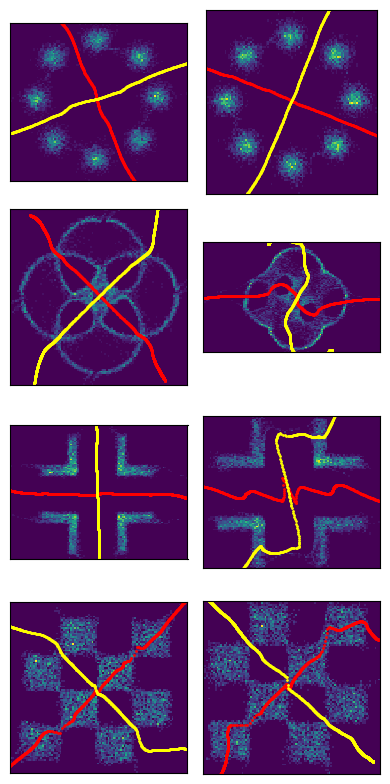
\includegraphics[angle=90, width=0.7\textwidth]{images/synthetic/symmetry_lines/symmetry_lines_all.png}
%     \caption{Symmetry lines from AbsoluteLayer for all datasets: first row is with learned q, second row with trained q}
%     \label{fig:symmetries_all}
% \end{figure}

\begin{figure}[H]
    \centering
    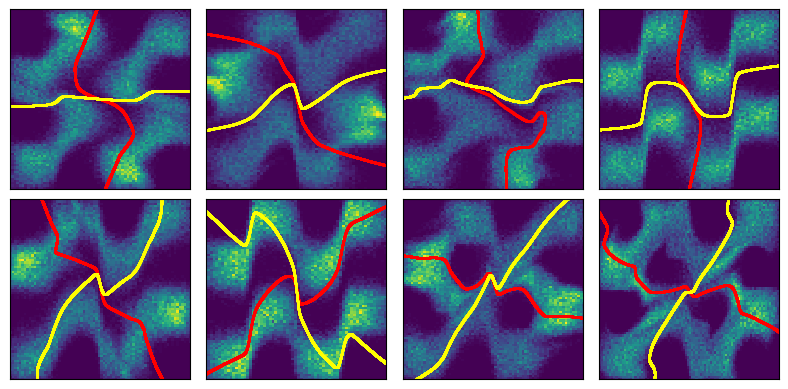
\includegraphics[width=0.9\textwidth]{images/synthetic/symmetry_lines/symmetry lines 3.png}
    \caption{Symmetry lines from \texttt{AbsoluteLayer} for Checkerboard after $100$ epochs. The symmetry lines are roughly correct and the datasets start to have the correct shape.}
    \label{fig:symmetries_checkerboard}
\end{figure}

\begin{figure}[H]
    \centering
    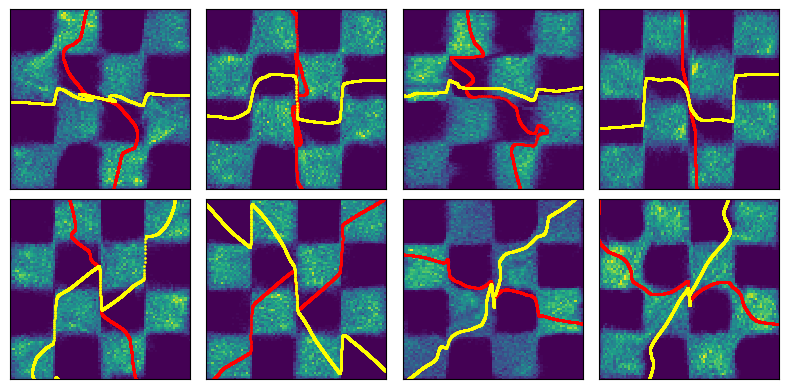
\includegraphics[width=0.9\textwidth]{images/synthetic/symmetry_lines/symmetry lines 4.png}
    \caption{Symmetry lines from \texttt{AbsoluteLayer} for Checkerboard after $1\,000$ epochs. Most of the datasets retain the original symmetry lines with only minor refinements, only one (row 1, column 2) changes them entirely.}
    \label{fig:symmetries_checkerboard_2}
\end{figure}

As we see, the learned symmetries are correct, albeit sometimes more complex than they need to be (diagonals would have sufficed).
They are also mostly unchanged after being established around $100$ epochs, just refined until the $1000$ epoch mark which contains correctly trained models. 

\asubsubsection{\texttt{AbsoluteLayer} -- Labeled}{Tomáš Sláma}

\textit{The results are taken from the \href{https://github.com/xiaoxiae/GNNFinal2024/blob/main/notebooks/abs\_conditional.ipynb}{notebooks/abs\_conditional.ipynb} notebook.}

Next, we took the labeled the datasets and modified the models to be conditional on the one-hot-encoding of the dataset labels.
Starting with the same models (baseline, abs, abs-trained) and datasets (n-gon, circles, corners, checkerboard) as the previous section, the results can be seen in Figure \ref{fig:abs-conditional}.

\begin{figure}[p]
    \centering
    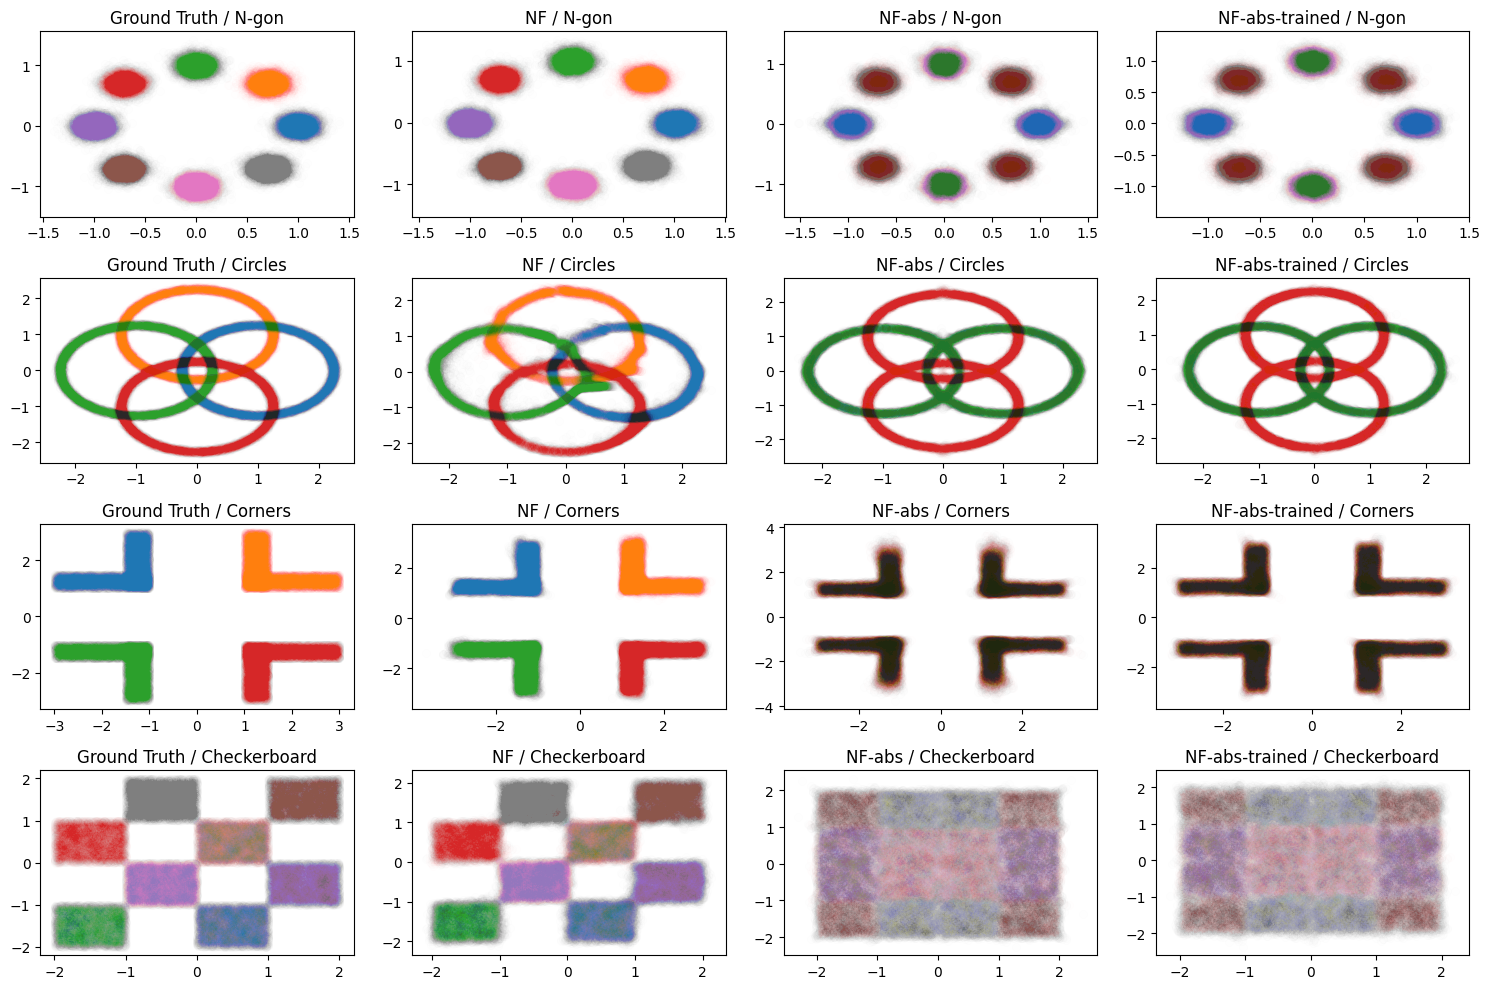
\includegraphics[width=.85\linewidth]{images/synthetic/abs-conditional.png}
    \caption{Comparison of methods for \textit{labeled} synthetic datasets; columns are same as Figure \ref{fig:abs-default}.}
    \label{fig:abs-conditional}
\end{figure}

\begin{figure}[p]
    \centering
    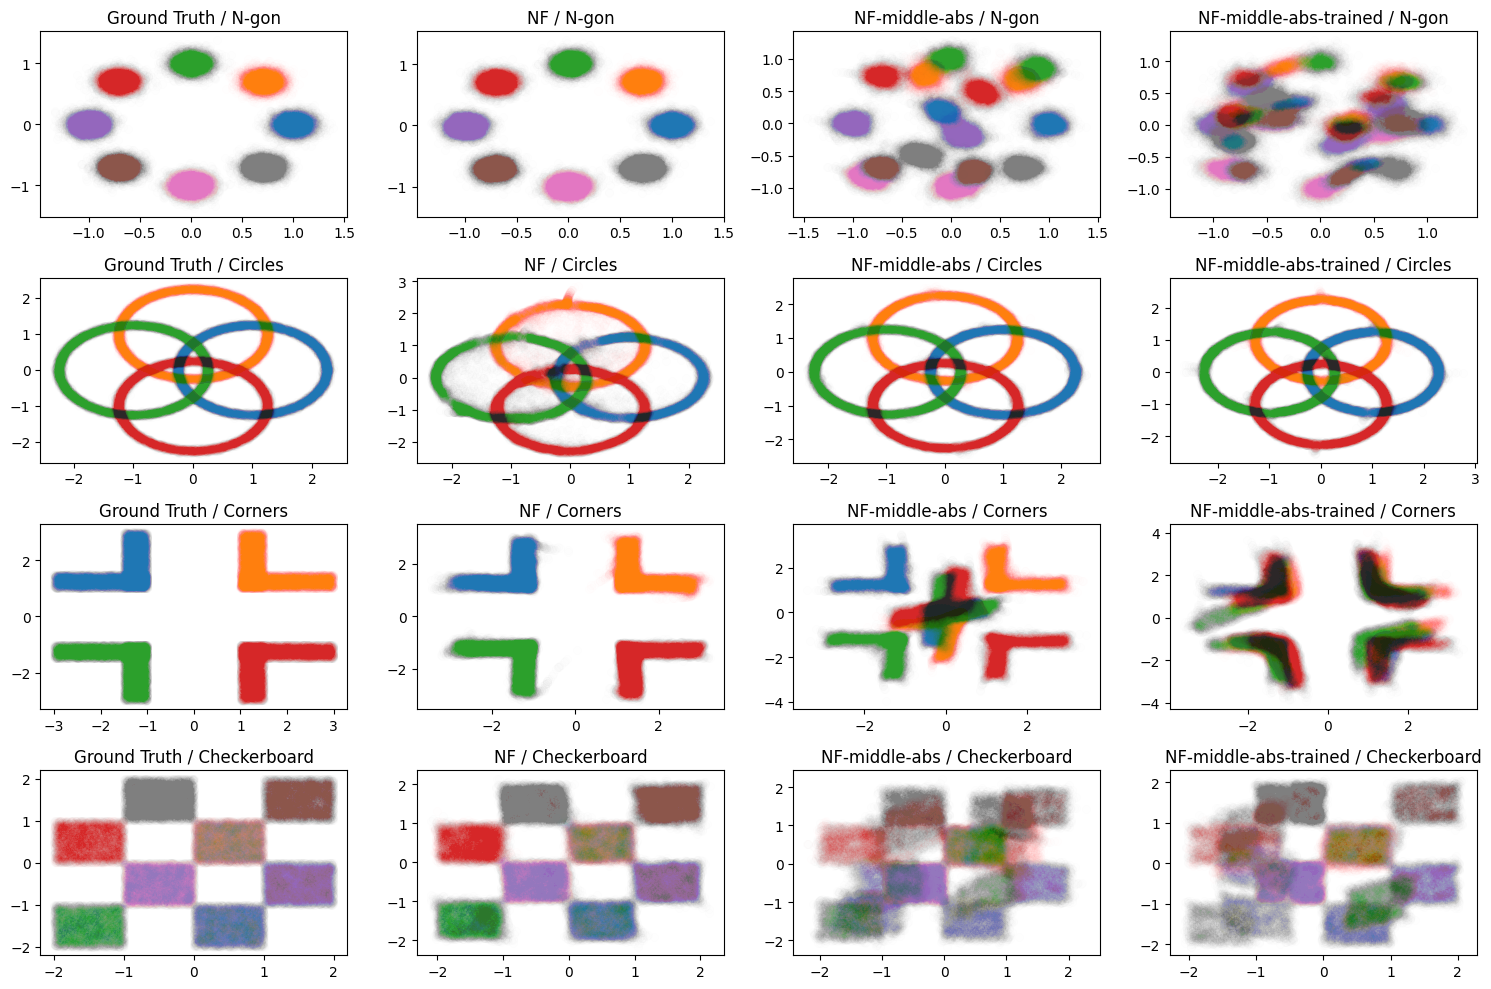
\includegraphics[width=.85\linewidth]{images/synthetic/abs-conditional-2.png}
    \caption{Comparison of methods for \textit{labeled} synthetic datasets; first two columns are same as Figure \ref{fig:abs-conditional}, last two are changed by moving the absolute layer in the middle.}
    \label{fig:abs-conditional-2}
\end{figure}


The models with the absolute layers suddenly become unusable, due to the fact that the datasets lose their symmetry. This is not solved by moving the absolute layer to the middle, as Figure \ref{fig:abs-conditional-2} shows.
\asubsubsection{\texttt{AugmentLayer}
-- Unlabeled}{Tomáš Sláma}

\textit{The results are taken from the \href{https://github.com/xiaoxiae/GNNFinal2024/blob/main/notebooks/augment.ipynb}{notebooks/augment.ipynb} notebook.}

The next experiment we chose to replicate is contained in appendix H.1 of the original paper, which compares a baseline normalizing flows network:

\begin{minted}{python}
(BijectiveLayer(2, [64] * 5), OrthonormalLayer(2)) x 3
BijectiveLayer(2, [64] * 5)
\end{minted}

with one that contains an \texttt{AugmentLayer} at the very beginning to make the dimensionality of all layers besides the last one increased:

\begin{minted}{python}
Augment(2, 4),
(BijectiveLayer(4, [64] * 5), OrthonormalLayer(4)) x 3
BijectiveLayer(4, [64] * 5)
\end{minted}

This should theoretically lead to better convergence, since the layers have more dimensions in which to optimize for the training values.
The results can be seen in Figure \ref{fig:augment}.

\begin{figure}[H]
    \centering
    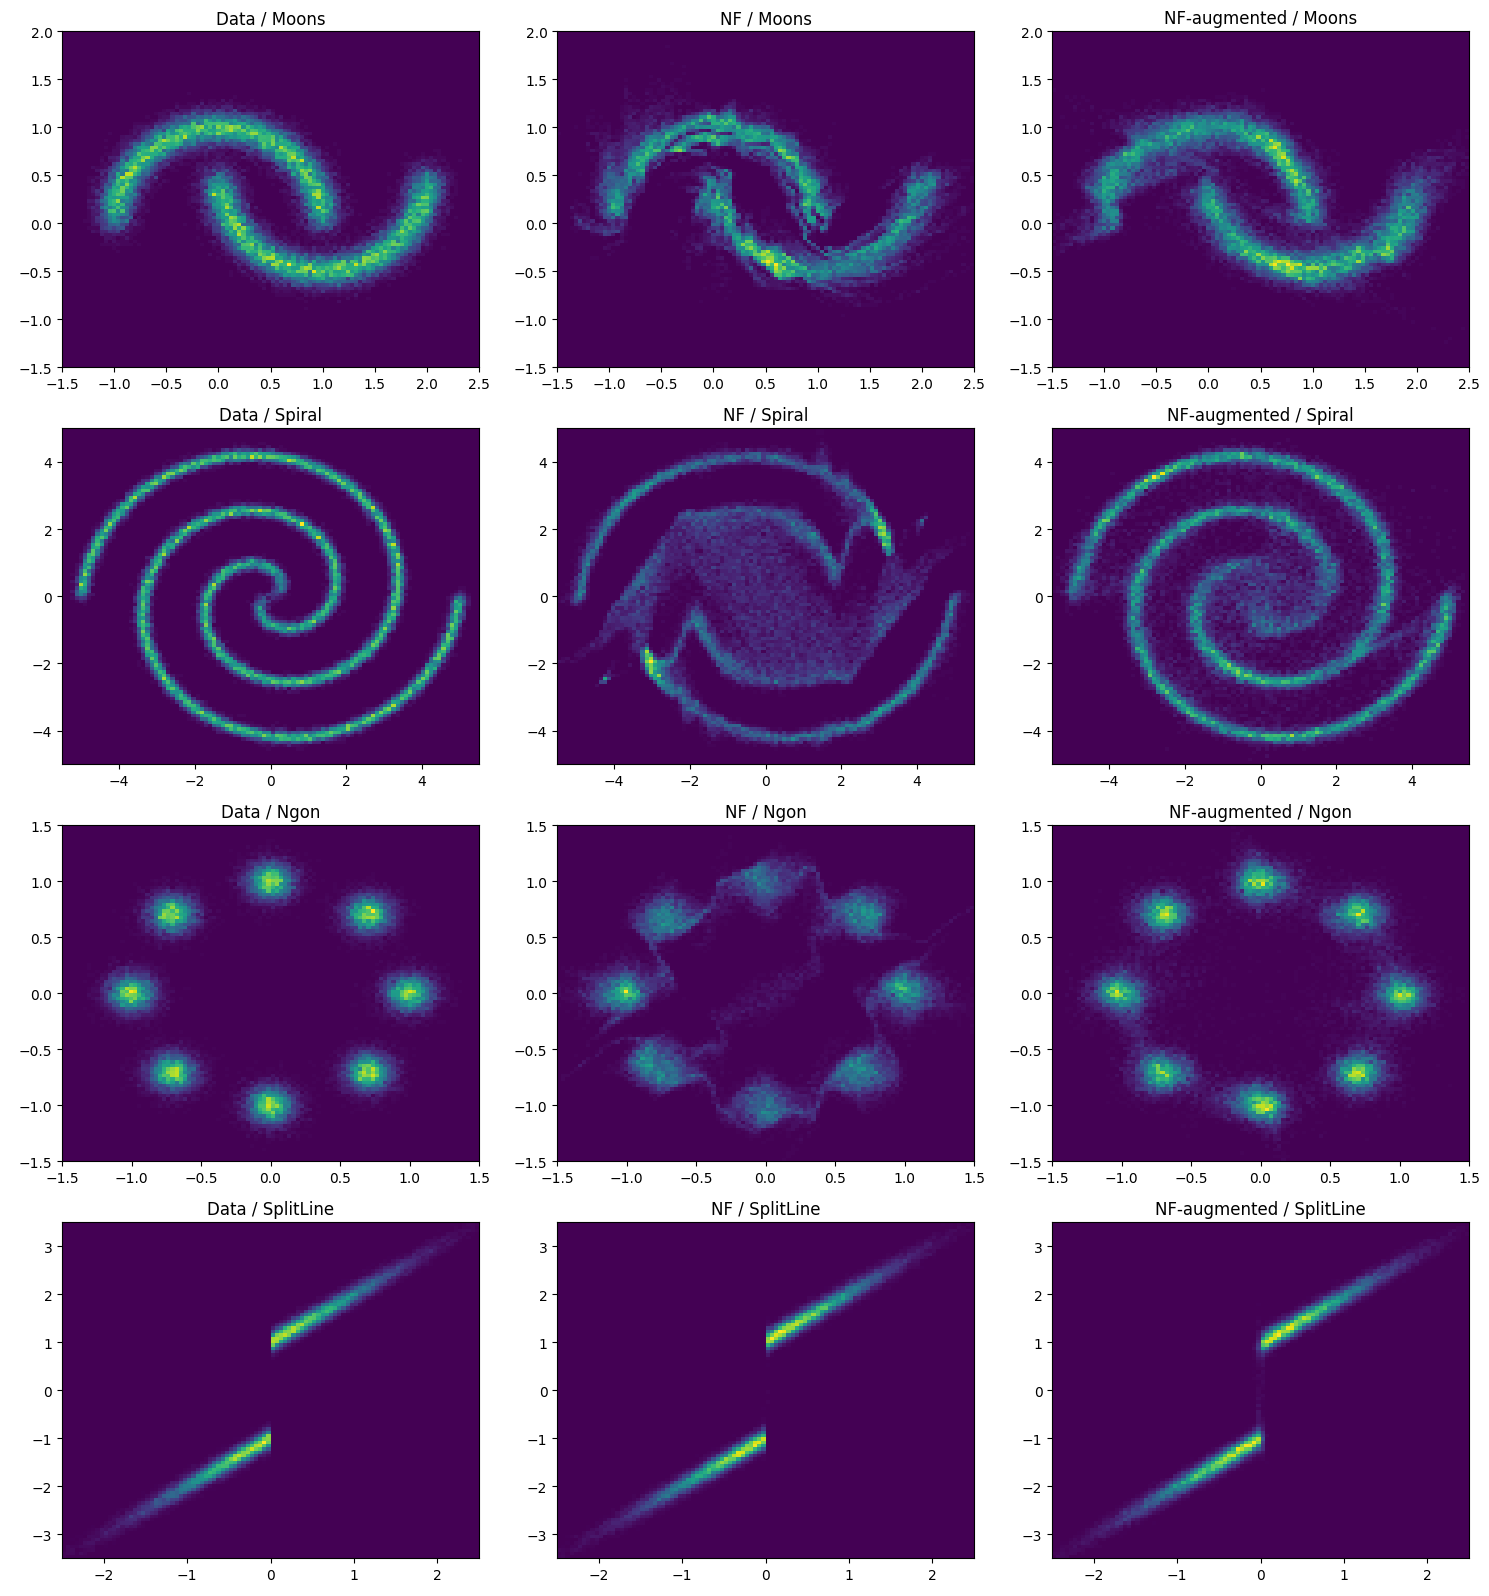
\includegraphics[width=.85\linewidth]{images/synthetic/augment.png}
    \caption{Five synthetic datasets (left column), along with a baseline NF network (middle column) and a network with an \texttt{AugmentLayer} at the beginning (right column).}
    \label{fig:augment}
\end{figure}

This is indeed the case and confirms the findings of the original paper.

\newpage

\asubsection{Point Cloud Data}{Maria Stickel}\label{sec:spatial_mnist}

\begin{figure}[p]
\centering
\begin{subfigure}[t]{.48\textwidth}
    \centering
    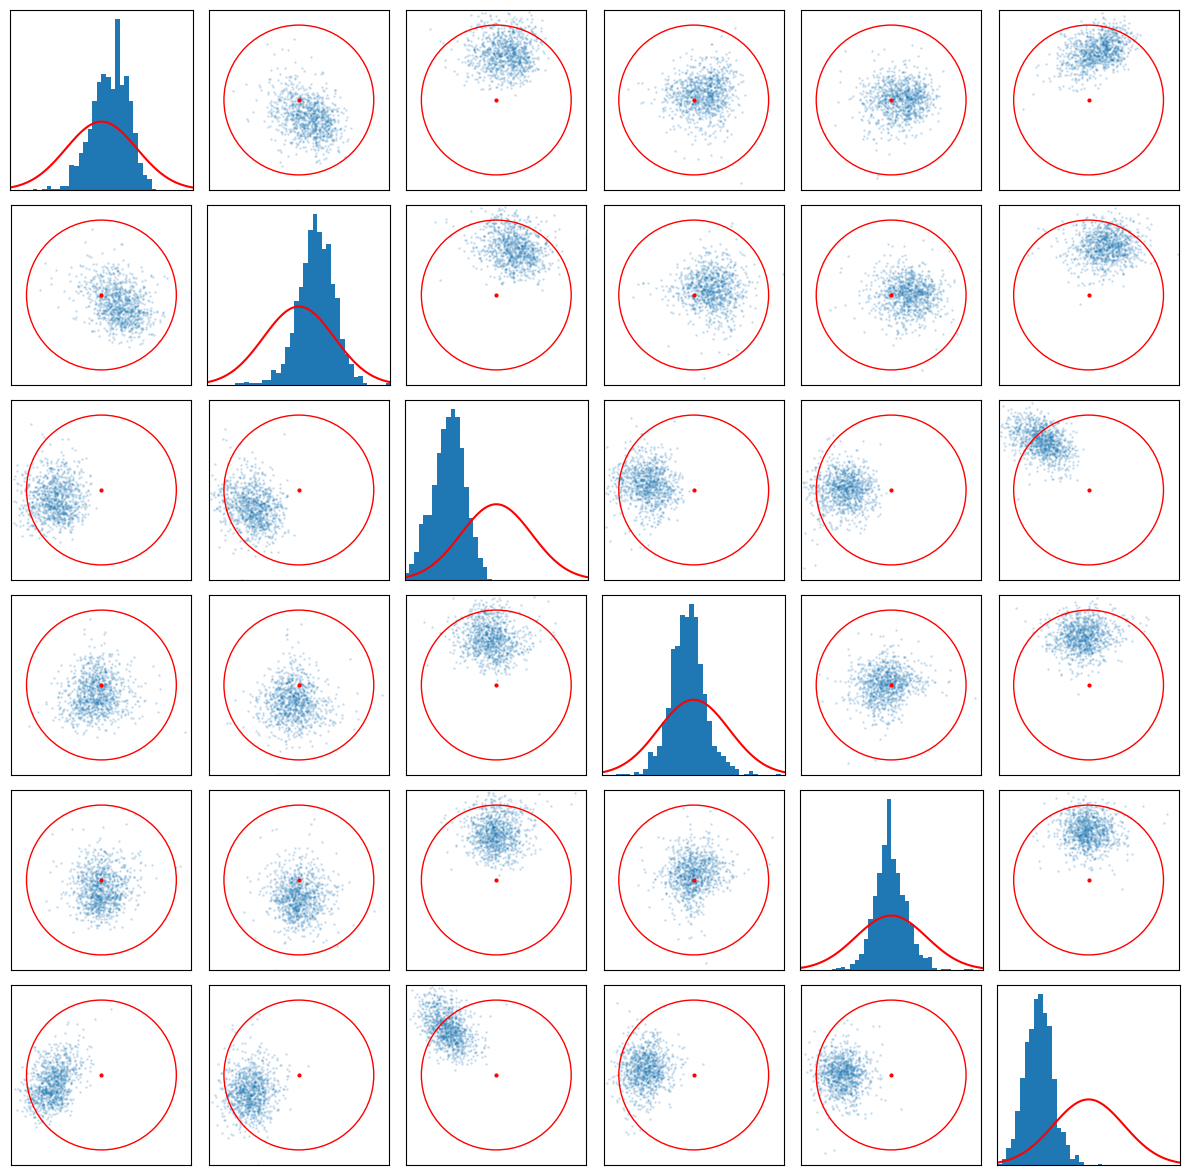
\includegraphics[width=\textwidth]{images/spatial_mnist/before_bij_layer_fix/calibration.png}
    \caption{One- and two-dimensional slices of the (N\textunderscore POINTS x 2)-dimensional latent distribution for the MNIST Point Cloud.}\label{fig:calibration_spatial_mnist_before}
\end{subfigure}
\hfill
\begin{subfigure}[t]{.48\textwidth}
    \centering
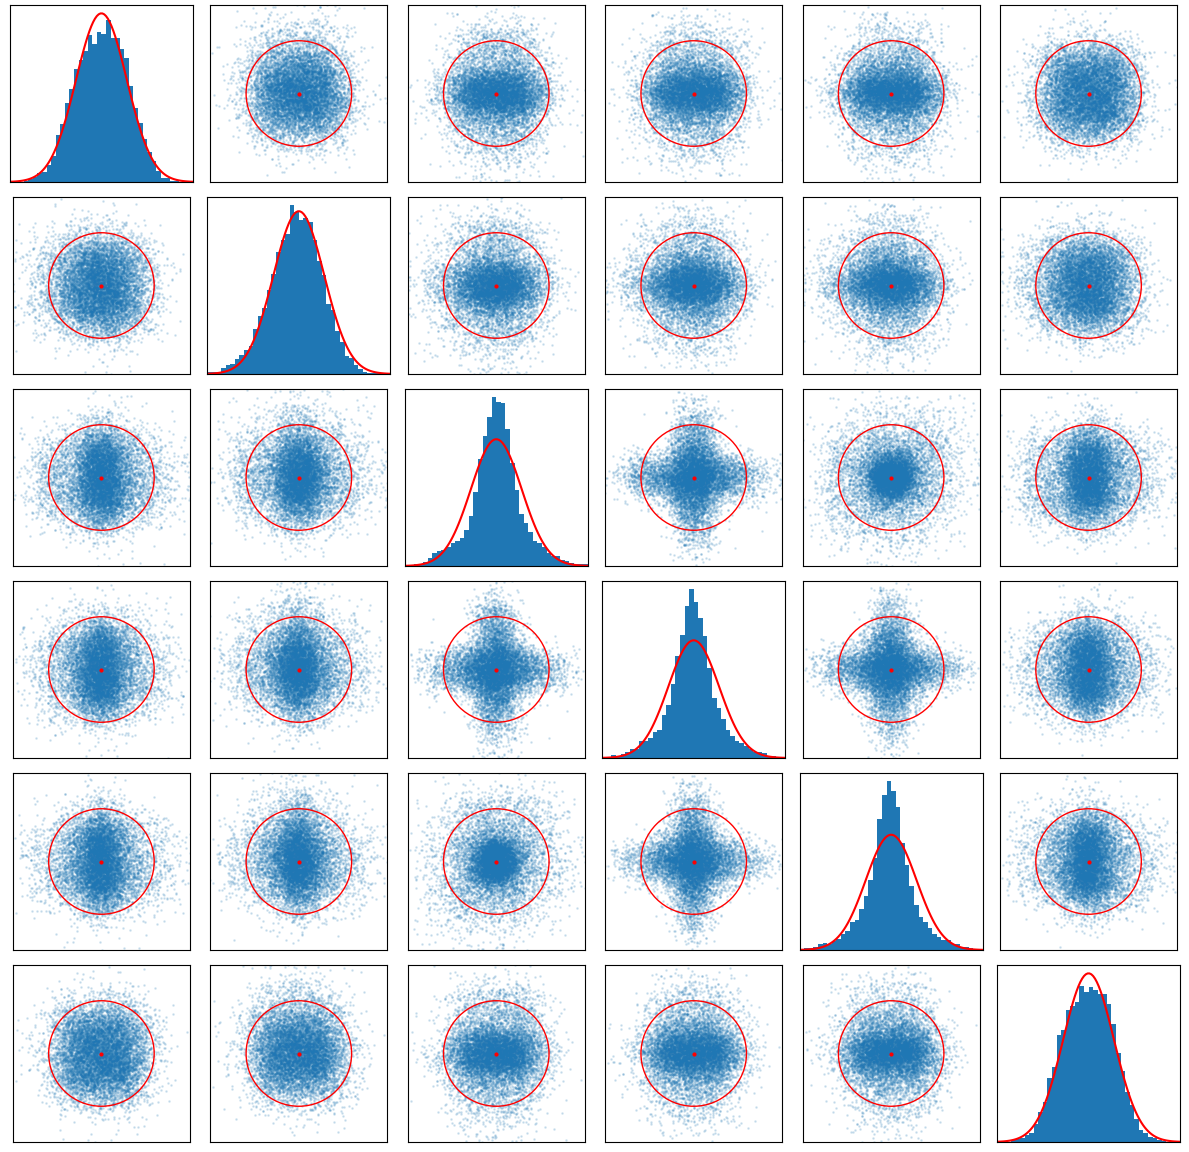
\includegraphics[width=\textwidth]{images/spatial_mnist/after_bij_layer_fix/code distribution.png}
    \caption{Code distribution for spatial MNIST after fixing the bijective layer.}
    \label{fig:spatial_mnist_code_after}
\end{subfigure}
\caption{Code distributions of SpatialMNIST model.}
\end{figure}

\begin{figure}[p]
    \centering
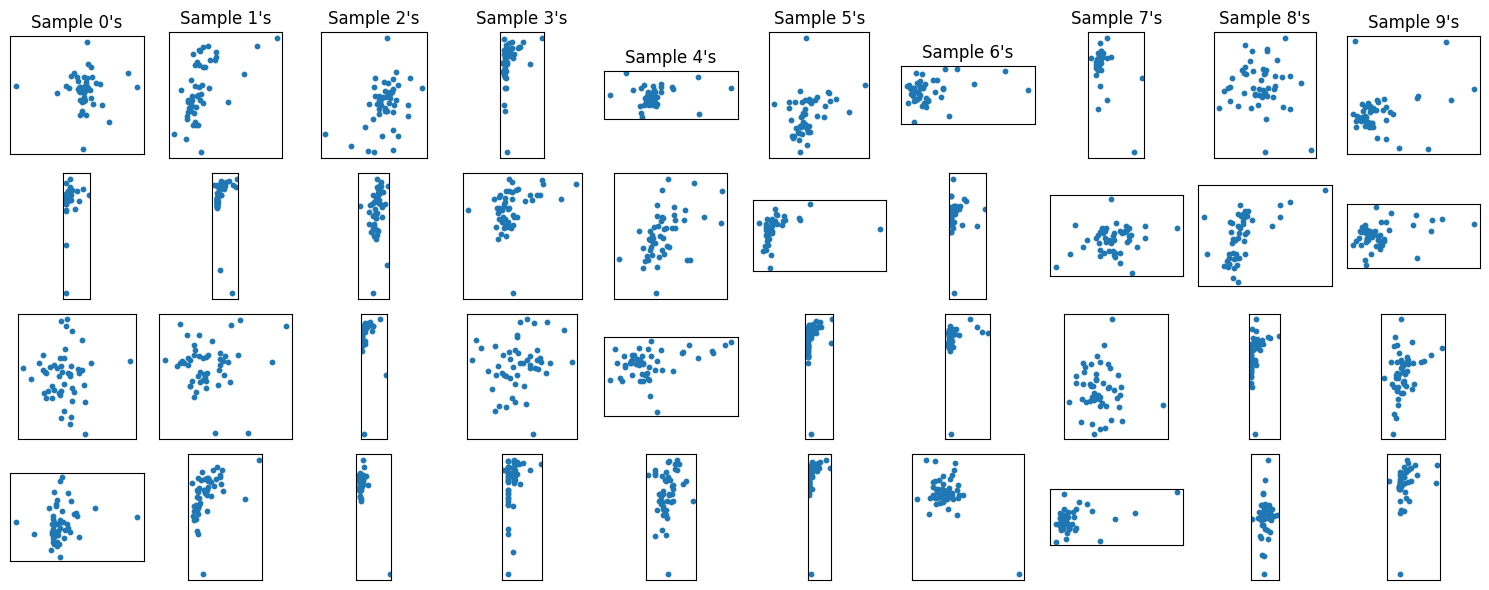
\includegraphics[width=0.95\textwidth]{images/spatial_mnist/after_bij_layer_fix/samples no ticks.png}
    \caption{Samples of our final spatial MNIST model}
    \label{fig:spatial_mnist_samples}
\end{figure}

\textit{The results are taken from the \href{https://github.com/xiaoxiae/GNNFinal2024/blob/main/notebooks/spatial_mnist.ipynb}{notebooks/spatial\textunderscore mnist.ipynb} notebook.}

\cite{nielsen2020survae} use parametrization by transformer networks (\cite{vaswani2023attention}) in their model architecture for the Point Cloud Data. As previously mentioned, we did not implement this feature, as we lack the knowledge about transformers (or rather the time to acquire a sufficient background of knowledge about their structure and application). We spent some time on researching transformer architectures, which the paper mentions in two (!) sentences without any further explanation of how they are applied in the architecture, although they used their own modified implementation for it. This research is not part of our architecture due to the fact that none of us have actually worked with transformers before and it proved to be too big of a topic to be learned and implemented that quickly. We thought about copying their transformer implementation, but using foreign code with nearly no knowledge on the underlying model is not a thing we wanted to do in a scientific research project.

We tried a different approach that didn't prove to be nearly as good as the paper, but then again, we ran into time issues. We report the results of our models. In the end, we decided to use the following architecture
\begin{minted}{python}
(
    PermuteAxesLayer((1, 0)), 
    BijectiveLayer((2, N_POINTS), [200, 200]), 
    PermuteAxesLayer((1, 0)),
    TranspositionLayer, 
    BijectiveLayer((N_POINTS, 2), [200, 200]), 
    PermutationLayer()
)   x 32,
ReshapeLayer((2, N_POINTS), (2 * N_POINTS,))
\end{minted}
where N\textunderscore POINTS is the number of points in the cloud. In each block we firstly permute in the first axis, i.e. re-order the list of points in the cloud. We apply a bijective transformation and permute again. Then we transpose the individual points in the cloud to ensure that the subsequent bijective transformation is applied on the vector entries skipped before (coordinate-wise). Another permutation completes the block. We reshape the data to enable easy sampling.

Before adjusting the bijective layer to this type of structured data, the results were bad. The standard deviation of the code distribution was measured to be 0.3879 which also aligns with the bad results shown in \ref{fig:calibration_spatial_mnist_before}. It should fulfill sigma=1, but one can only wonder whether this could have been achieved through more training with such an unfit model. The samples were equally bad.

Fixing the bijective layer and training in the architecture described above significantly improved the results. The code distribution resembles the normal distribution with sigma 1, see Figure \ref{fig:spatial_mnist_code_after}.

Training was done with the following hyperparameters:  batch-size=200, test-size=1\,000, epochs=100\,000 and initial learning rate=$10^{-3}$ with decay parameter gamma=0.97 applied every 1\,000 steps. The model in \cite{nielsen2020survae} was trained on a single GPU for 40 hours. The loss plot could lead one to think that the model has converged but could also be related to the learning rate decay. Needless to say we would have liked to train for a longer period and different hyperparameters, but there was no time. The model has not learned the distribution of the spatial MNIST dataset, see \ref{fig:spatial_mnist_samples}.


\asubsection{Image Data}{Jannis Heising}\label{sec:image_data}

\textit{The results were generated using the \href{https://github.com/xiaoxiae/GNNFinal2024/blob/main/notebooks/mnist784.ipynb}{notebooks/mnist784.ipynb} notebook.}

As with the preceding two sections, our initial goal was to replicate the paper's training setup as accurately as possible, i.e. to train a SurVAE with a dequantization layer and max-pooling layers on the CIFAR-10, ImageNet32, and ImageNet64 datasets. This was very ill-advised since the authors report a training time of two weeks for their simplest model, which was infeasible for our project, alas we only noticed the issue during the experiment setup. As a result, we chose to train a smaller SurVAE with similar architecture on a simpler dataset, namely MNIST784. As a benchmark, we planned to compare its FID score with state-of-the-art models for that dataset.

In contrast to the paper, we chose to make our model conditional, which was only feasible due to our simpler dataset. The condition is a one-hot encoding of the digits 0-9. This means that a fully trained model would be able to create images of specific digits as opposed to arbitrary ones.

We chose the following baseline architecture:

\begin{minted}{python}
DequantizationLayer(),
(BijectiveLayer(784, [200, 200]), OrthonormalLayer(784)) x 5,
MaxPoolingLayer(784, 2),
(BijectiveLayer(196, [200, 200]), OrthonormalLayer(196)) x 5,
MaxPoolingLayer(196, 2),
(BijectiveLayer(49, [200, 200]), OrthonormalLayer(49)) x 5,
MaxPoolingLayerWithOverlap(49, 3, 2),
(BijectiveLayer(9, [200, 200]), OrthonormalLayer(9)) x 5
\end{minted}

In other words, the model uses four different scales (28x28, 14x14, 7x7, 3x3) and 5 steps per scale, and all nested neural networks have two hidden layers of size 200. We chose to end up with a fairly low-dimensional latent distribution because the information contained in the images is very small - one of ten digits with slightly varying styles.

On the other hand, each downscaling step should be gentle in the sense that we do not want to loose too much data at once, hence four scales. The choice of twenty bijective layers was based on the assumption that the model could be slightly simpler than those described in the paper, which had twenty-four.\footnote{We only list the parameter choices we deem interesting here. The exact setups for the tests in this section are documented in the repository, should more detail be desired. They are always stored as ``\texttt{setup.txt}" in the appropriate directories.}

For proper hyperparameter testing, each choice of parameters should ideally be tested several times and updated systematically. However, the given time frame of three weeks did not allow for such rigorousness for a model of the given complexity. Thus, we properly tested each configuration only once (plus small preliminary tests of a few epochs each) and iteratively chose the next experiment mainly based on the outcome of its predecessor. A ``proper test" consisted of a training time of around eight hours on an Nvidia~GTX~970 graphics card.

\textbf{Experiment 1:} In our first attempt, we somewhat foolishly used a reconstruction loss term because the NLL loss for the max-pooling layers was implemented incorrectly. We also disabled the dequantization layer to make the reconstruction loss more expressive. The samples presented in Figure~\ref{fig:mnist_run_1_samples} show that this approach was unwise.

\textbf{Experiment 2:} After fixing the problematic NLL loss terms, we trained another model with the exact architecture shown above. The new samples (Figure~\ref{fig:mnist_run_2_samples}) seemed more promising, but still far from perfect. The drastic difference between the top and bottom halves of the sampled images stems from the first (i.e. last during generation) bijective layer, in which the upper half constitutes the skip connection and only the lower half is altered. This perhaps suggests that the layer in question is being trained much more slowly than the other ones, although we were unable to find a cause for such a phenomenon. Furthermore, while the learned latent distribution did resemble a normal distribution, it had the wrong standard deviation, as shown in Figure~\ref{fig:mnist_run_2_latent_distr}. At any rate, the loss graph (Figure~\ref{fig:run_2_loss}) seemed to suggest that this model had reached its peak.

\begin{figure}
\centering
\begin{subfigure}[t]{.48\textwidth}
    \centering
    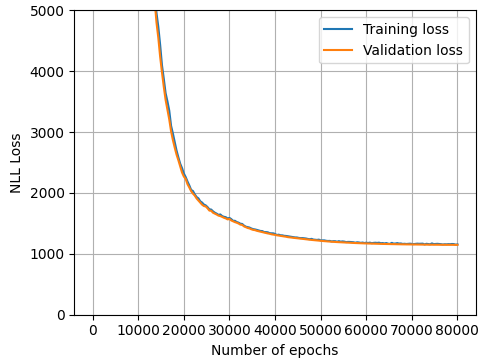
\includegraphics[width=\textwidth]{images/mnist_maxpooling/run_2_loss.png}
    \caption{Loss graph of the second experiment. The model seems to have mostly stagnated.}
    \label{fig:run_2_loss}
\end{subfigure}
\hfill
\begin{subfigure}[t]{.48\textwidth}
    \centering
    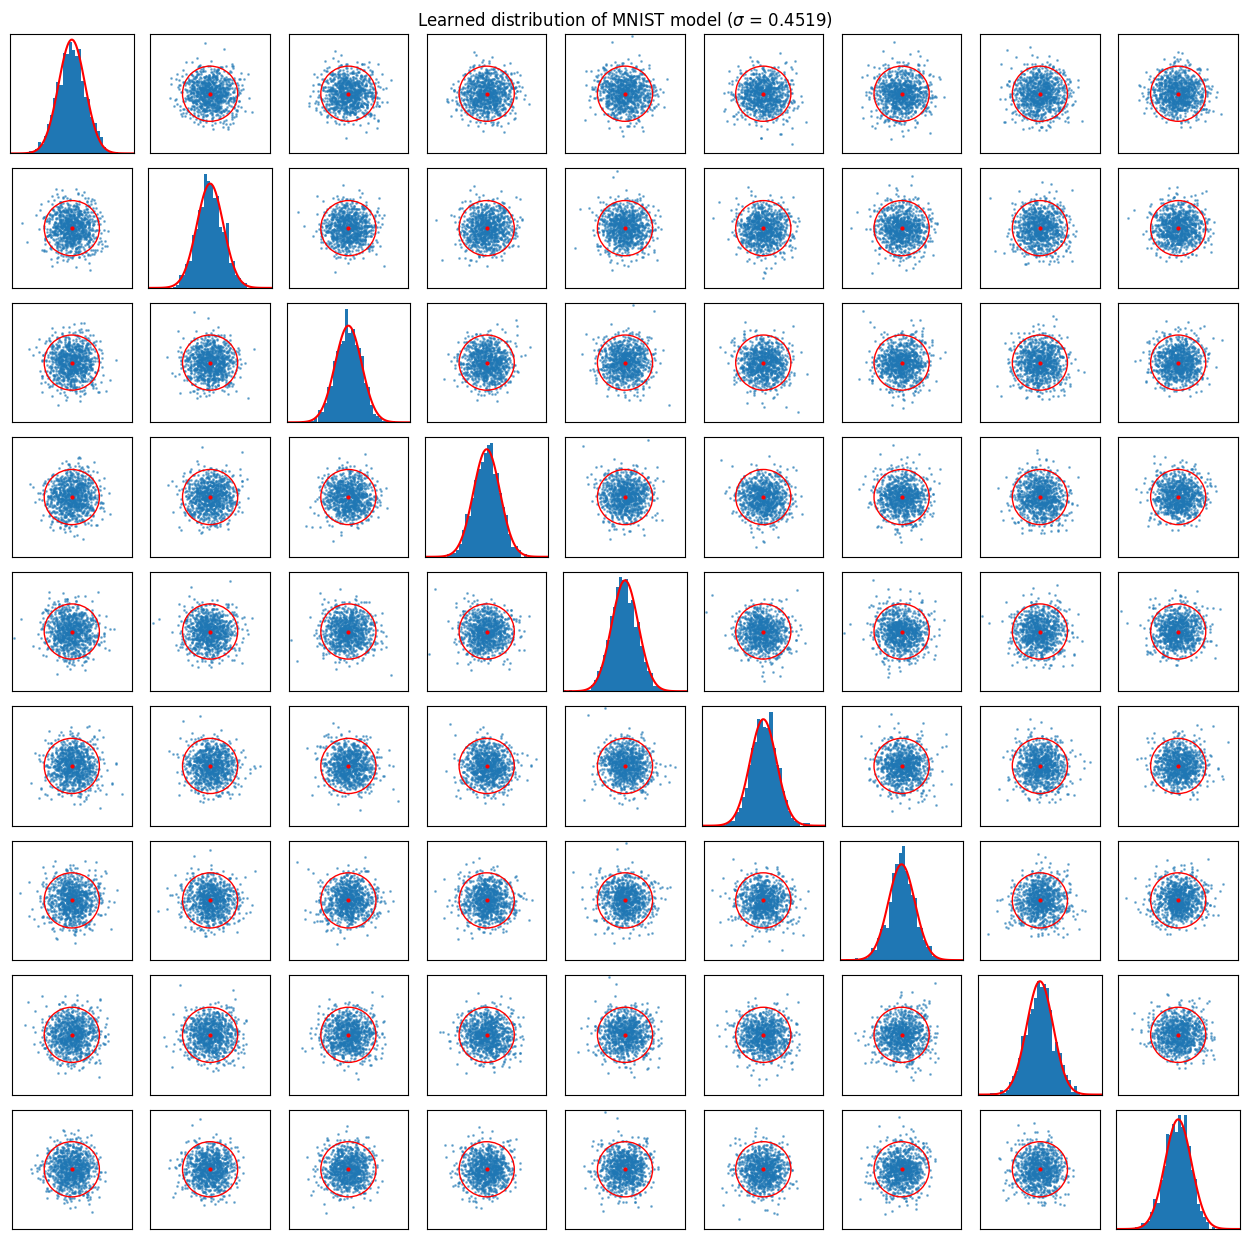
\includegraphics[width=.8\textwidth]{images/mnist_maxpooling/run_2_latent_distr.png}
    \caption{One- and two-dimensional slices of the nine-dimensional latent distribution. It clearly resembles a normal distribution with standard deviation around 0.45 (shown in red; the circles indicate the 90\%-threshold) instead of the desired 1.}
    \label{fig:mnist_run_2_latent_distr}
\end{subfigure}
\caption{Results from experiment 2.}
\end{figure}

\textbf{Experiment 3:} Next, we increased the model architecture to six steps per scale (instead of five) and increased the hidden layer sizes of the nested neural networks in the first scale to \verb|[200, 500, 200]| (from \verb|[200, 200]|). In an attempt to speed-up training, we decreased the hidden layer sizes in the last scale to \verb|[200]| (from \verb|[200, 200]|). Figure~\ref{fig:mnist_run_3_samples} illustrates that these changes did not help.

While our previous attempts at explaining either of the two major problems of the second test - slow \texttt{BijectiveLayer} training and small standard deviation - were fruitless, we now managed to trace both back to the same root cause. We want to explain how we actually found the issue in the hopes that it might help readers when debugging their own implementation. To start, let us take another look at the NLL loss (cf. Section~\ref{sec:nf_explanation}):

\begin{align*}
\text{NLL} &= \mathbb{E}_{X \sim p^*(X)} [-\log(p(X))]\\
&= \mathbb{E}_{X \sim p^*(X)} [-\log(q(f(X) \cdot |\det \mathcal{J}_{f}|)]\\
&\approx \underbrace{- \frac{1}{N} \sum_{i=1}^N \log(q(f(X_i))}_{=: A} - \underbrace{\frac{1}{N} \sum_{i=1}^N \log(|\det \mathcal{J}_{f, i}|)}_{=: B}
\end{align*}

Roughly speaking, term $A$ is responsible for pulling samples in the code distribution towards the origin, whereas term $B$ makes sure the translation between latent and data distribution is good. Seeing that our model excelled at the former and struggled with the latter, we were confident that the balance between the two was off. Term $A$ is very simple and was quickly ruled out as the culprit. Thus, we revisited term $B$, i.e. the log-likelihood computation of the layers. As we had similar problems with other experiments that did not involve max-pooling layers, it was clear that the issue had to lie within the \texttt{BijectiveLayer} class. Carefully examining our implementation, we realized that our coefficient generation was faulty. Recall that the bijective layer performs a computation of the form (cf. Section~\ref{sec:bijective})

\[
\tilde{X} = s \cdot X + t,
\]

where the coefficients $s$ and $t$ are the output of a feed-forward neural network. The shape of the vector $X$ is \verb|(N, D)|, where $N$ is the batch size and $D$ is the data size. It should be clear that $s$ and $t$ ought to have the same shape, however we only sampled $s$ of shape \verb|(N, 1)|, i.e. we applied the same coefficient to all data dimensions for each batch entry. This alone is quite bad as it greatly limits the transformative power of the layer, but it wouldn't have caused the issues we observed, had we not simultaneously assumed for the log-likelihood computation that $s$ has the correct shape. This resulted in the log-likelihood term being $D$ times too small, creating the aforementioned imbalance between the loss terms $A$ and $B$.

\textbf{Experiment 4:} Having resolved this slight inconvenience, we repeated the setup of the second test as it had yielded the best results up to that point. However, we did change two parameters: Firstly, we decreased the batch size from 1,000 to 200. Both of these values were chosen rather arbitrarily as we did not have the time to conduct rigorous hyperparameter test as mentioned above. The decrease massively sped up training, going from roughly 2.8 to just over 8.2 epochs per second, and seemed not to dampen the training merit of each epoch in equal and opposite magnitude, in other words it was an unequivocally good change. Secondly, we increased training time from around 8 to 11 hours split into sessions of 3 and 8 hours. This change stemmed from the general principle that ``more training is better" and the fact that our schedules happened to allow for the additional training.

Disappointingly, the samples (Figure~\ref{fig:mnist_run_4_samples}) were still bad, but we did find a plausible explanation for it: Throughout all of these experiments, we had been using learning rate decay and basically eyeballing the values for it.\footnote{Again, the exact values are recorded in the repository.} When plotting the learning rate together with the test loss during training (Figure~\ref{fig:mnist_run_4_loss_vs_lr}), one senses a strong correlation between the two.

\begin{figure}
\centering
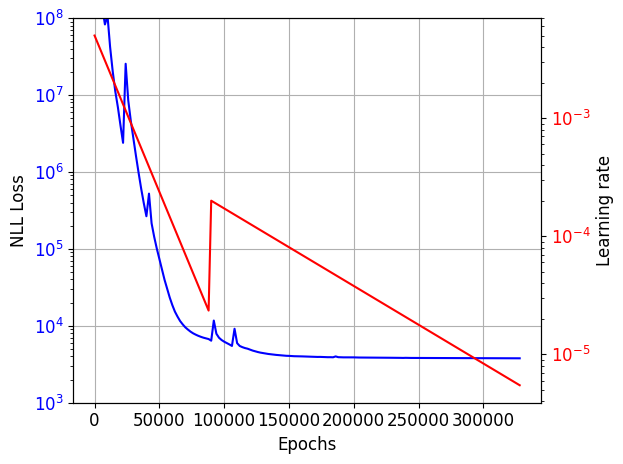
\includegraphics[width=.65\textwidth]{images/mnist_maxpooling/run_4_loss_vs_lr.png}
\caption{Negative log-likelihood loss (blue, log-scale) and learning rate (red, log-scale) from the fourth test. The irregularity in both lines at 88,000 epochs indicates the start of the second training session. The somewhat faster loss decrease right afterwards seems to stem from the increased learning rate.}
\label{fig:mnist_run_4_loss_vs_lr}
\end{figure}

\begin{figure}
\centering
\begin{subfigure}[t]{0.45\textwidth}
    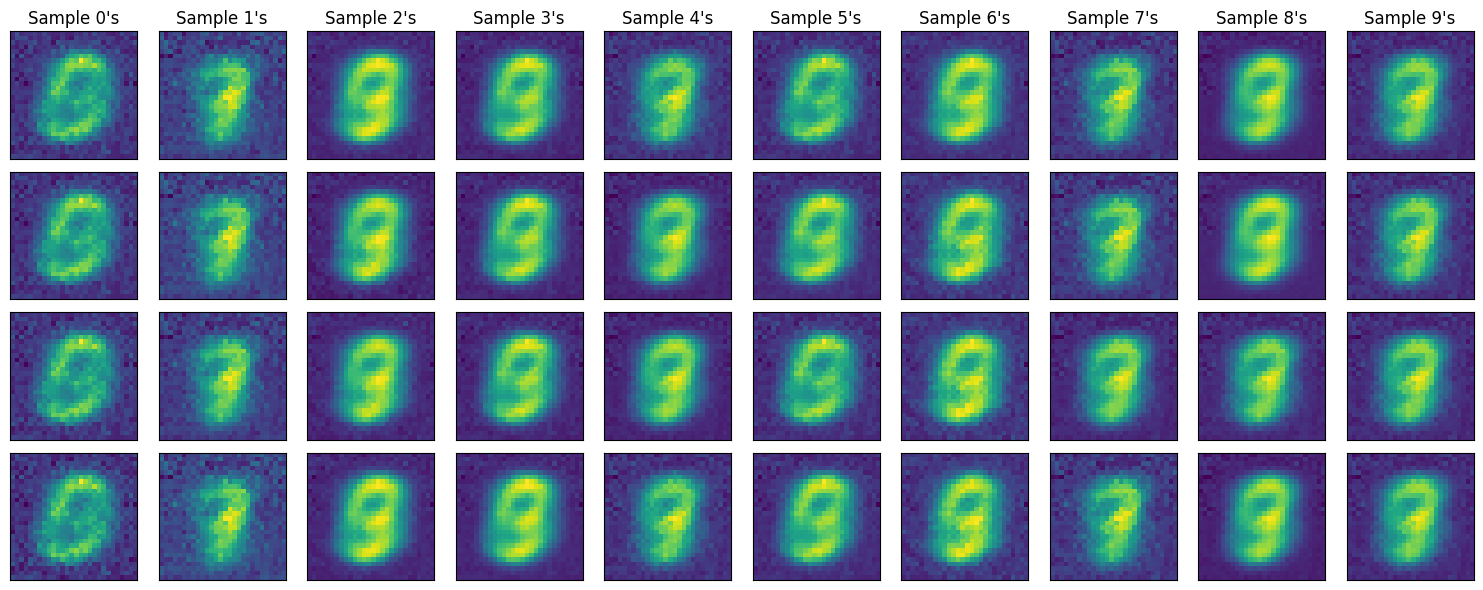
\includegraphics[width=\textwidth]{images/mnist_maxpooling/run_1_samples.png}
    \caption{\footnotesize Samples from the first experiment. Each digit (column) was sampled four times (row). The images are barely distinguishable and mostly resemble a blur of all digits.}
    \label{fig:mnist_run_1_samples}
\end{subfigure}
\hfill
\begin{subfigure}[t]{0.45\textwidth}
    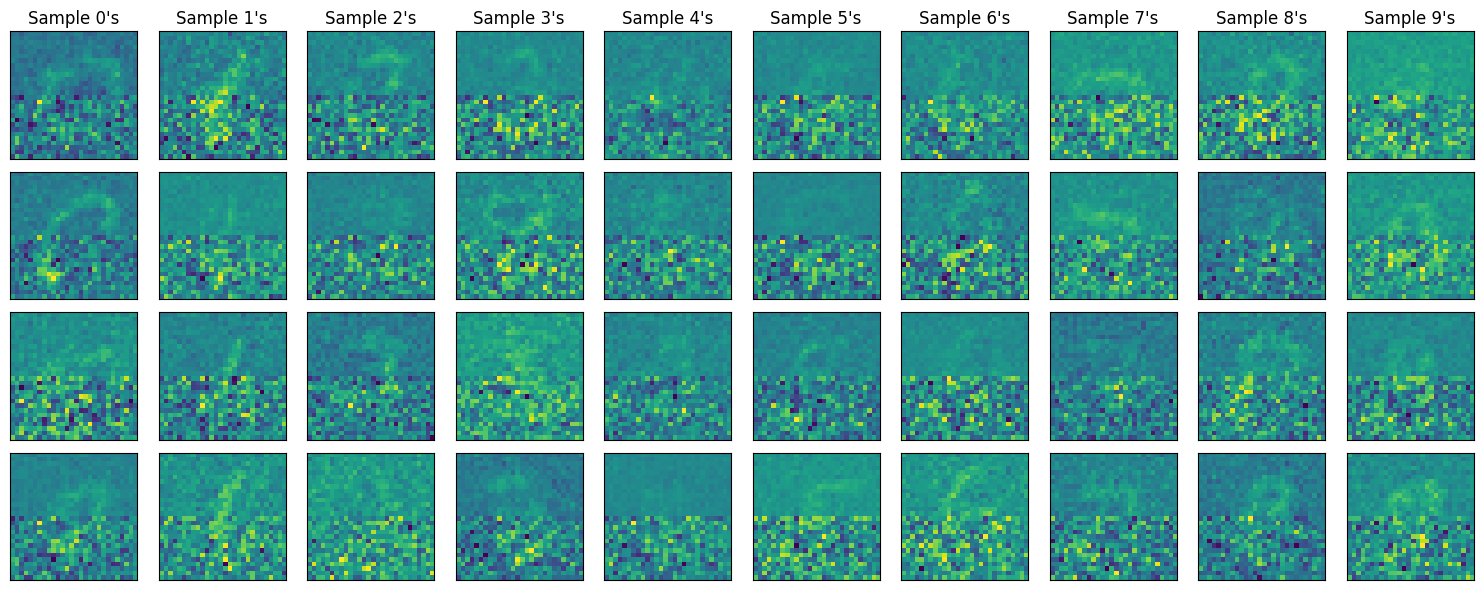
\includegraphics[width=\textwidth]{images/mnist_maxpooling/run_2_samples.png}
    \caption{\footnotesize Samples from the second experiment. The images are split in-two, with the top half showing vaguely correct shapes and the lower half being mostly gibberish.}
    \label{fig:mnist_run_2_samples}
\end{subfigure}\\
\vspace{.5em}
\begin{subfigure}[t]{0.45\textwidth}
    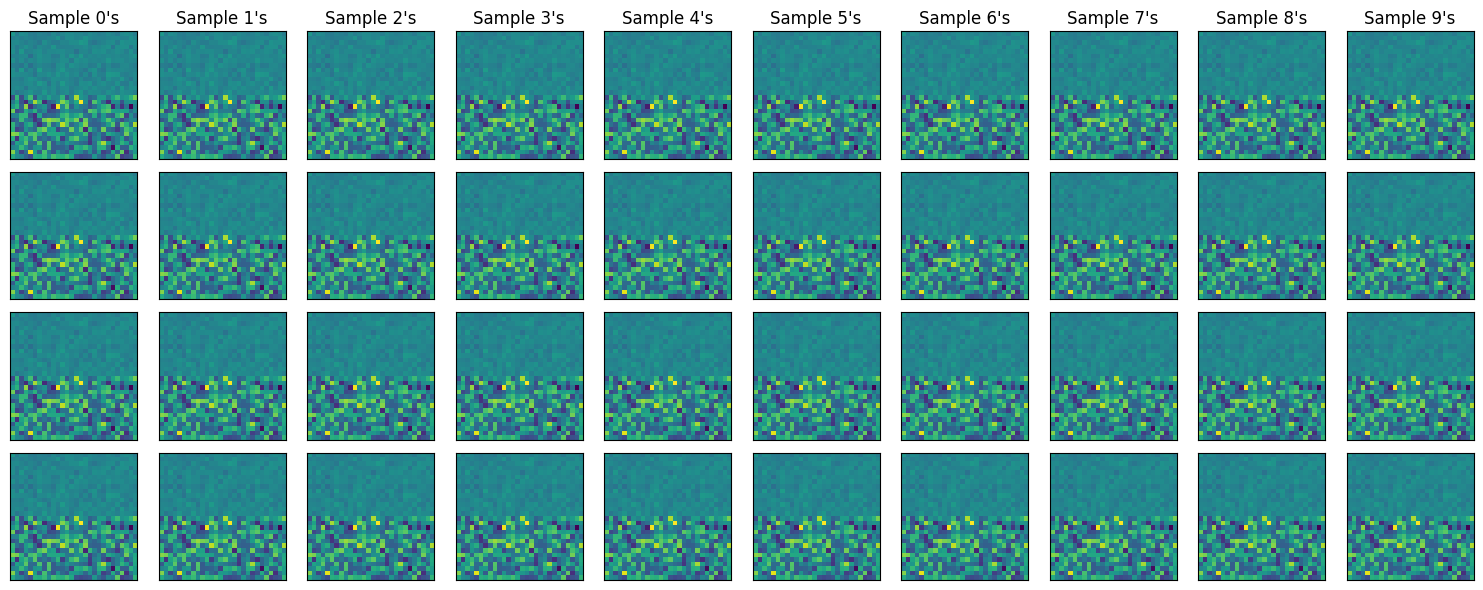
\includegraphics[width=\textwidth]{images/mnist_maxpooling/run_3_samples.png}
    \caption{\footnotesize Samples from the third experiment. The model did not converge after eight hours of training and the half-split conundrum persists.}
    \label{fig:mnist_run_3_samples}
\end{subfigure}
\hfill
\begin{subfigure}[t]{0.45\textwidth}
    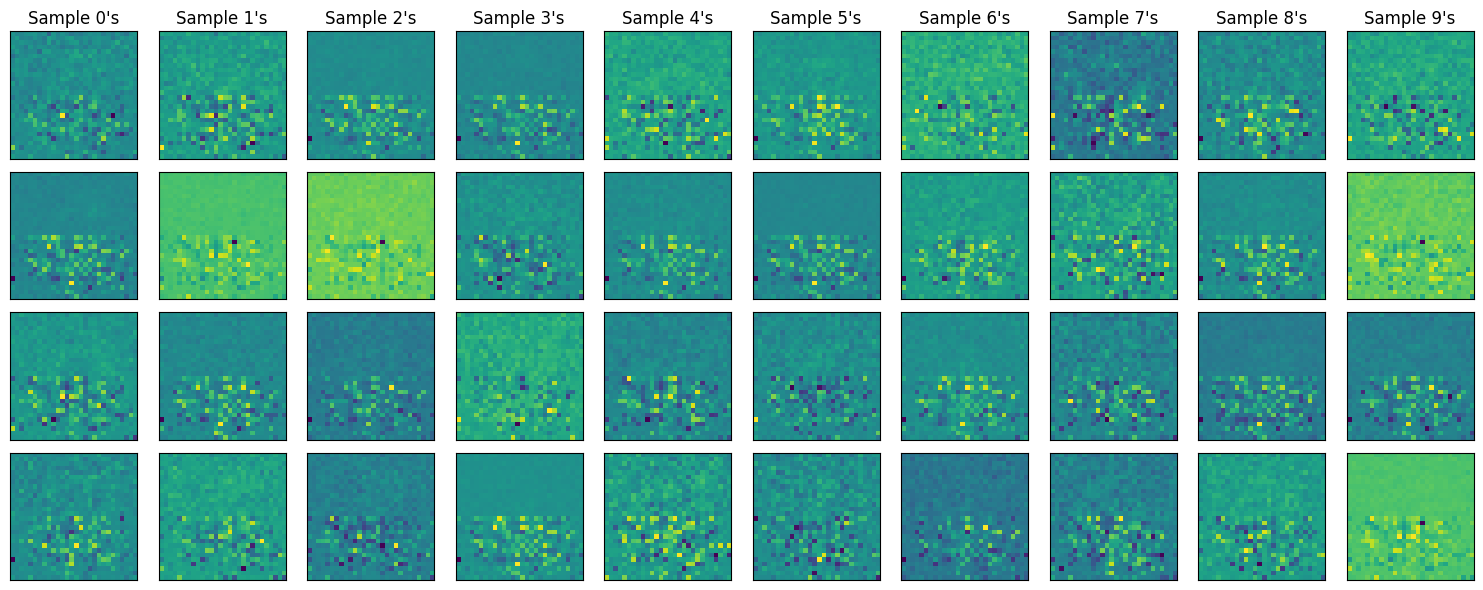
\includegraphics[width=\textwidth]{images/mnist_maxpooling/run_4_samples.png}
    \caption{\footnotesize Samples from the fourth experiment. There is no trace of digit shapes and the samples are still bi-regional, although notably less so.}
    \label{fig:mnist_run_4_samples}
\end{subfigure}
\caption{Samples from the MNIST experiments.}
\label{fig:mnist-all-samples}
\end{figure}

\textbf{Experiment 5:} From Figure~\ref{fig:mnist_run_4_samples}, we deduced that a constant learning rate of $10^{-4}$ should be ideal. We chose the model trained for 50,000 epochs from the previous test as the starting point for training and kept all other parameters as before. Figure~\ref{fig:mnist_4_vs_5} illustrates the impact of the higher learning rate: Initially, the model did learn faster, however its final performance was only marginally better; its samples were indistinguishable from those of the previous experiment. Furthermore, training seemed to be less stable, with the loss curve exhibiting significantly more spikes than before.

\begin{figure}
\centering
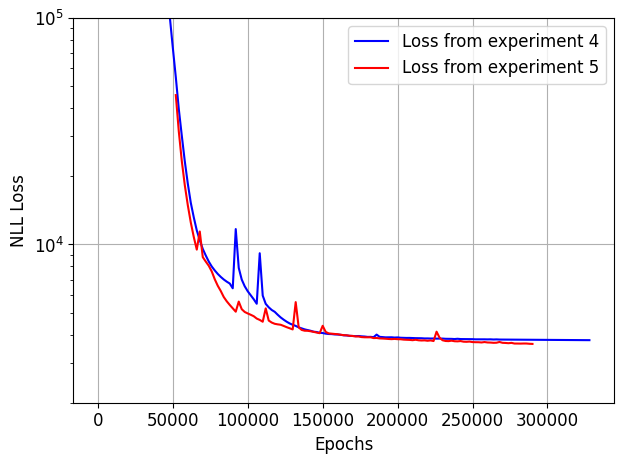
\includegraphics[width=.7\textwidth]{images/mnist_maxpooling/run_4_vs_5.png}
\caption{Validation loss from the fourth and fifth experiment.}
\label{fig:mnist_4_vs_5}
\end{figure}

From this result, we postulate that the chosen architecture was not expressive enough for the task. Unfortunately, we did not have time to conduct further experiments. Were we to resume our tests, we would like to use models with more bijective layers and larger nested networks, and we would like to measure how changing the latent dimensionality impacts the results.

It does not make sense to compare our work to the state-of-the-art using FID, seeing as our samples are unrecognizable.


\newpage
\asubsection{Parameter Degeneracy}{Jannis Heising}

Since this section explores an application of SurVAEs not discussed in the paper we are trying to replicate, the experiments described here were given less attention and, crucially, less time. As a result, many results are bad simply due to not being trained for long enough.

\asubsubsection{SBI}{Jannis Heising}\label{sec:sbi}

\textit{The results were generated using the \href{https://github.com/xiaoxiae/GNNFinal2024/blob/main/notebooks/sir.ipynb}{notebooks/sir.ipynb} notebook.}

The initial goal of our experiments involving parameter degeneracy was to assess whether the SurVAE architecture could be designed to cope with degenerate SBI models. To this end, we created a baseline by reimplementing exercise 1 from sheet 4 using both our own solution and snippets as well as general ideas from the sample solution. The exercise in question concerned the most basic SIR model described in Section~\ref{sec:sir_data}. We chose the following architecture for all experiments on this basic system:

\begin{minted}{python}
(BijectiveLayer(3, [150, 150]), OrthonormalLayer(3)) x 30
\end{minted}

Additionally, we equipped the SurVAE with a summary network $h$, which is a simple feed-forward neural network that condenses the conditional input - the observation data - into a more usable form for the SurVAE layers. We chose the layer sizes of $h$ to be \verb|[200, 200, 200, 100]| based on prior testing.

For the degenerate data, we replaced $\lambda$ by two new parameters $\lambda_1$ and $\lambda_2$ as explained in Section~\ref{sec:background_param_degen}. Initially we chose the exact same SurVAE architecture as before for this data, including that of the summary network, except that the bijective and orthonormal layers now act on four instead of three dimensions. This was to create a benchmark of how well the standard NF model performs on degenerate data to later compare to more sophisticated models.

\textbf{Experiment 1:} To get our bearings, we simply wanted to recreate the results from the exercise sheet and, ideally, show that the standard NF performed badly on degenerate data. We trained both the basic and the degenerate model (i.e. the model trained on the degenerate dataset) until convergence with underwhelming results.

The calibration diagrams and code distributions (Figure~\ref{fig:sir_run_1}) show that our models did not learn the correct distribution. As it turned out, this test used the faulty implementation of the \texttt{BijectiveLayer} as discussed in Section~\ref{sec:image_data}, so bad results were to be expected.

\begin{figure}[t]
\centering
\begin{subfigure}{\textwidth}
    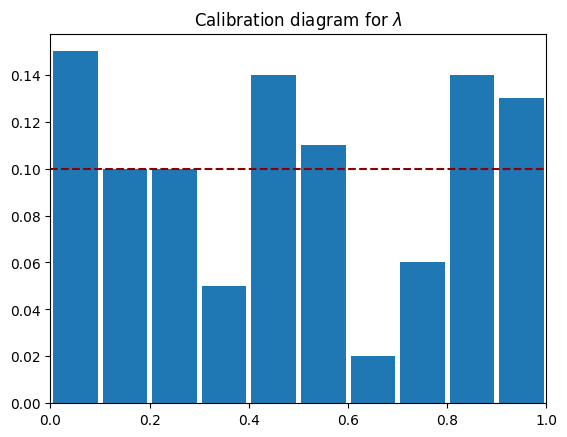
\includegraphics[width=.23\textwidth]{images/sbi_sir/run_1/basic calib lambda.png}
    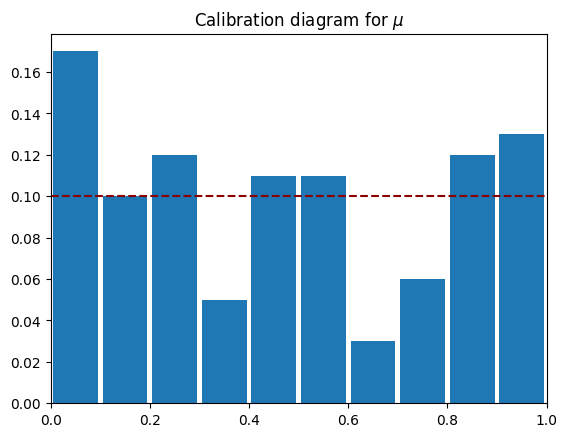
\includegraphics[width=.23\textwidth]{images/sbi_sir/run_1/basic calib mu.png}
    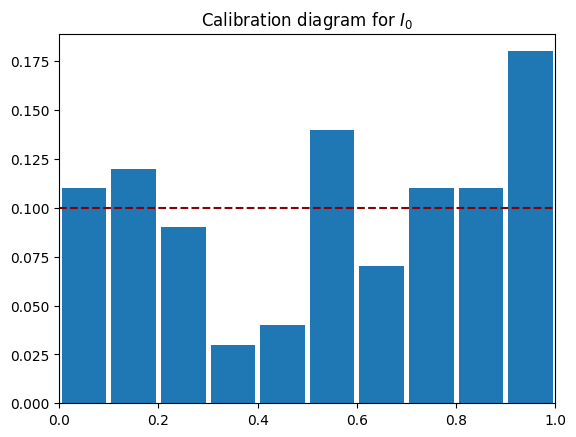
\includegraphics[width=.23\textwidth]{images/sbi_sir/run_1/basic calib I_0.png}
    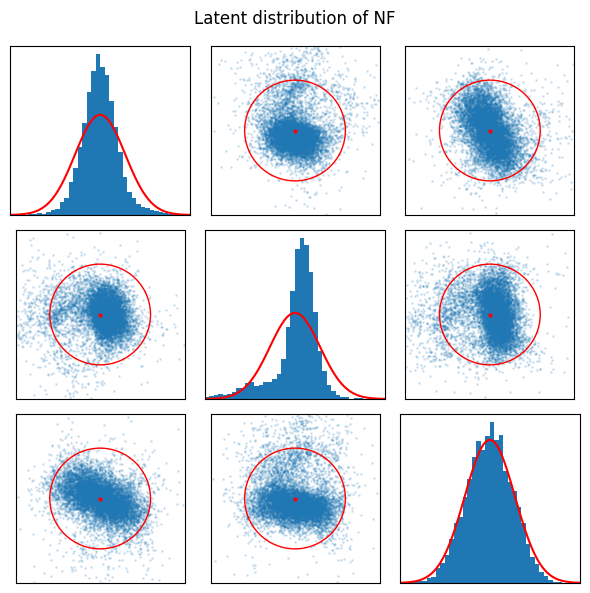
\includegraphics[width=.23\textwidth]{images/sbi_sir/run_1/basic code distribution.png}
    \caption{Calibration diagrams ($\lambda$, $\mu$, and $I_0$, respectively) and code distribution of basic model from the first test.}
\end{subfigure}

\begin{subfigure}{\textwidth}
    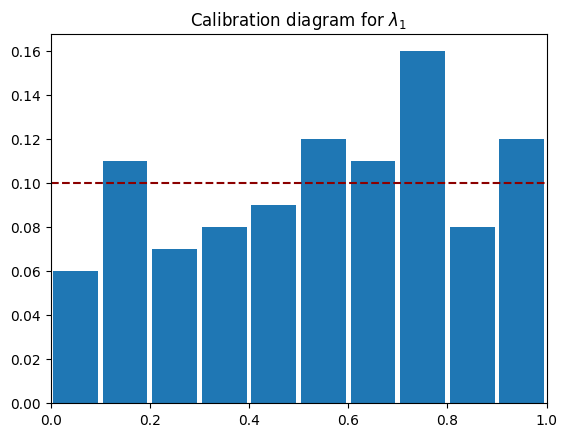
\includegraphics[width=.19\textwidth]{images/sbi_sir/run_1/degen calib lambda1.png}
    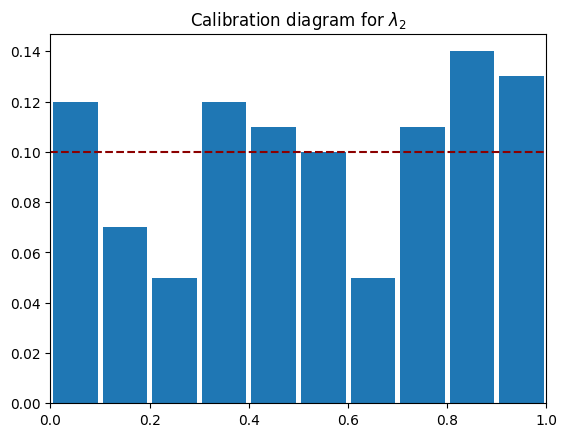
\includegraphics[width=.19\textwidth]{images/sbi_sir/run_1/degen calib lambda2.png}
    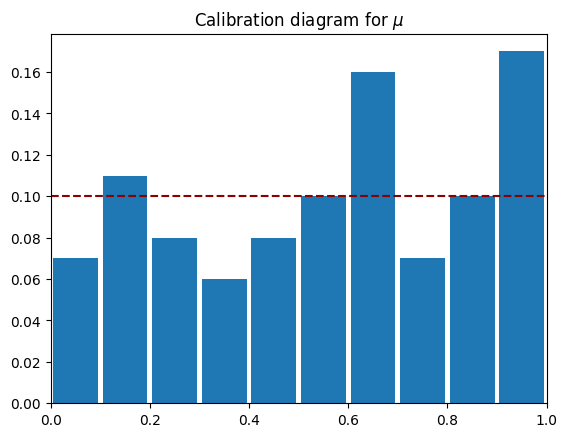
\includegraphics[width=.19\textwidth]{images/sbi_sir/run_1/degen calib mu.png}
    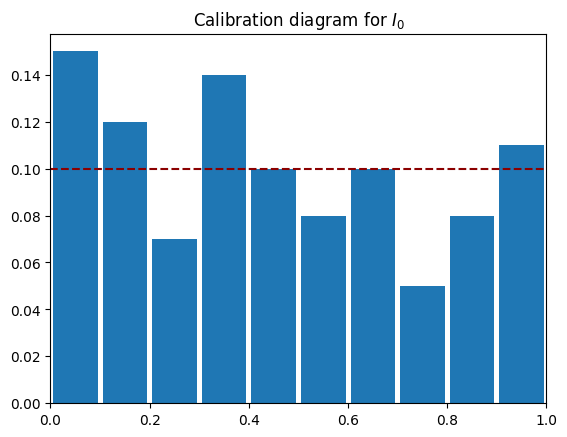
\includegraphics[width=.19\textwidth]{images/sbi_sir/run_1/degen calib I_0.png}
    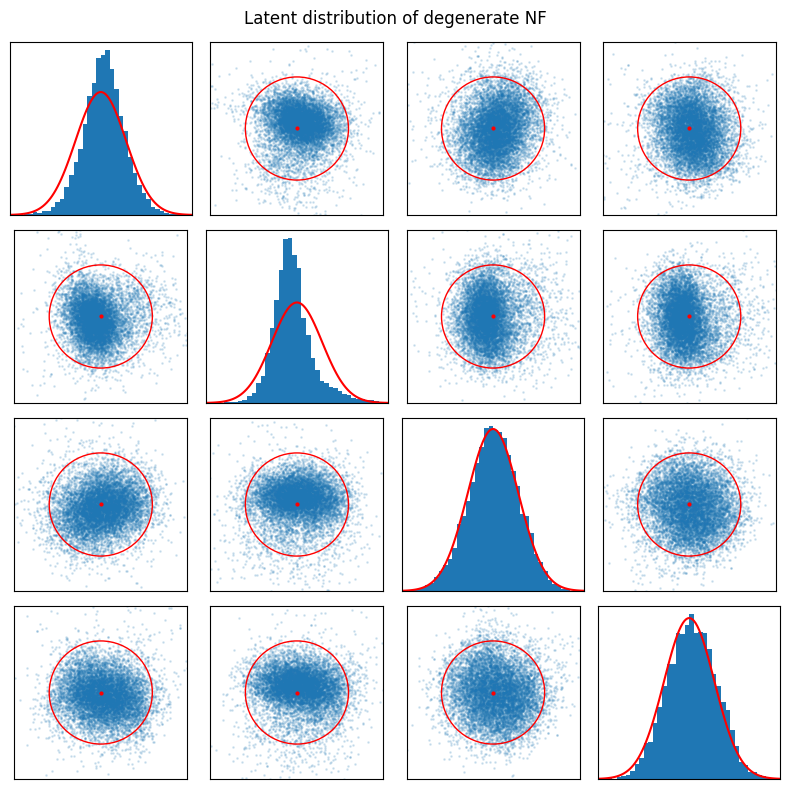
\includegraphics[width=.19\textwidth]{images/sbi_sir/run_1/degen code distribution.png}
    \caption{Calibration diagrams ($\lambda_1$, $\lambda_2$, $\mu$, and $I_0$, respectively) and code distribution of degenerate model from the first test.}
\end{subfigure}
\caption{Evaluation data from the first test.}
\label{fig:sir_run_1}
\end{figure}

\textbf{Experiment 2:} Having fixed \texttt{BijectiveLayer}, we repeated the first test, although we did not have the time to let the models train until convergence. To still get a fair comparison, both models were trained on the exact same hyperparameters, in particular on the same number of epochs (2000 in this case). The results (Figure~\ref{fig:sir_run_2}) were quite surprising:

\begin{figure}[ht]
\centering
\begin{subfigure}{\textwidth}
    \centering
    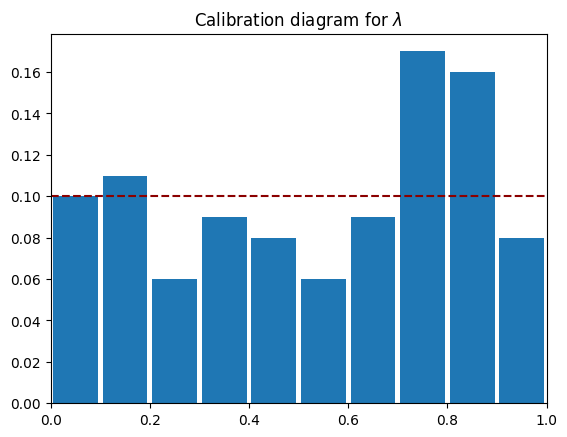
\includegraphics[width=.23\textwidth]{images/sbi_sir/run_2/basic calib lambda.png}
    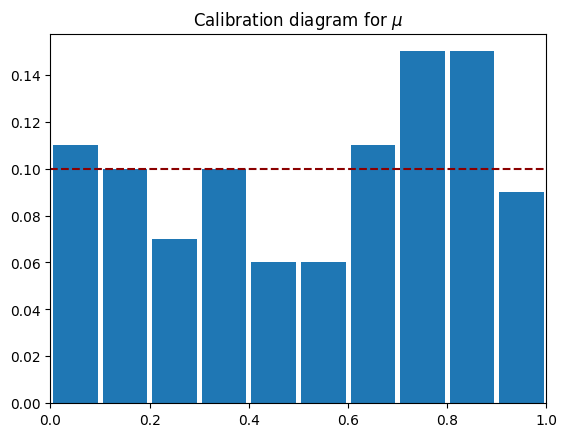
\includegraphics[width=.23\textwidth]{images/sbi_sir/run_2/basic calib mu.png}
    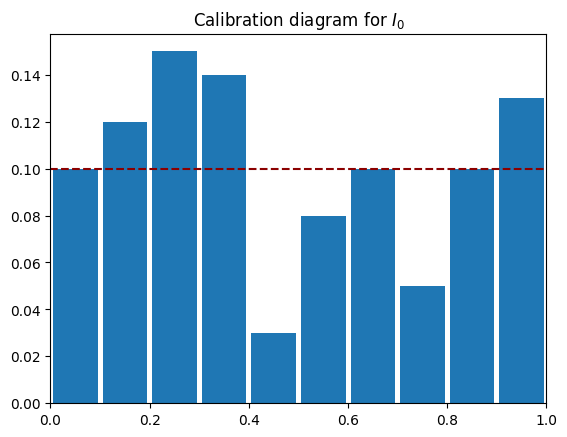
\includegraphics[width=.23\textwidth]{images/sbi_sir/run_2/basic calib I_0.png}
    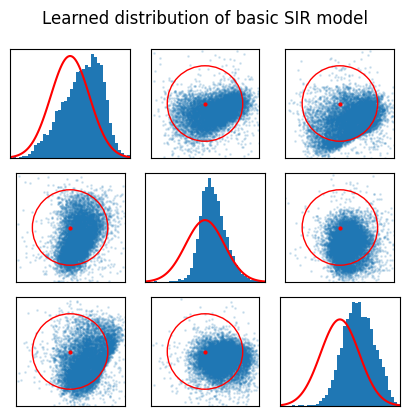
\includegraphics[width=.23\textwidth]{images/sbi_sir/run_2/basic code distribution.png}\\
    \vspace{.5em}
    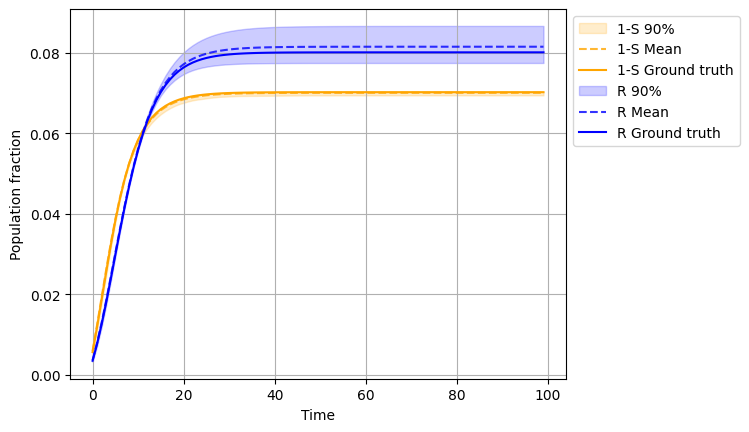
\includegraphics[width=.325\textwidth]{images/sbi_sir/run_2/basic resim 1.png}
    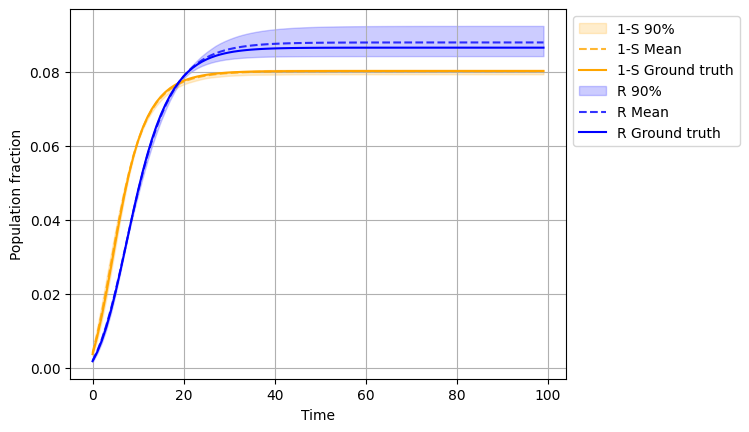
\includegraphics[width=.325\textwidth]{images/sbi_sir/run_2/basic resim 2.png}
    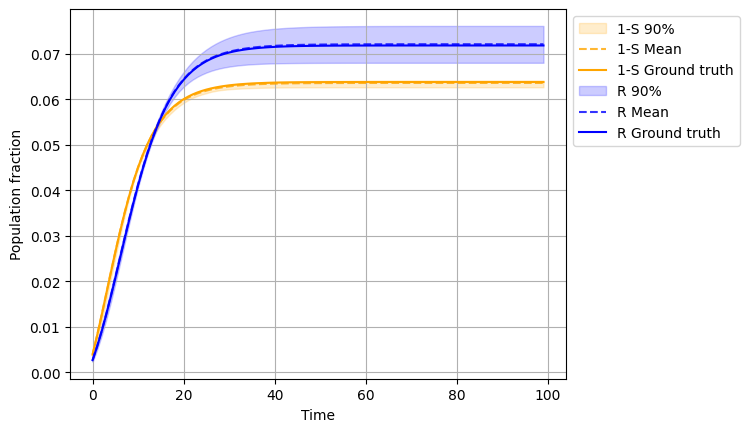
\includegraphics[width=.325\textwidth]{images/sbi_sir/run_2/basic resim 3.png}
    \caption{Calibration diagrams ($\lambda$, $\mu$, and $I_0$, respectively), code distribution and three resimulations of basic model from the second test.}
\end{subfigure}

\begin{subfigure}{\textwidth}
    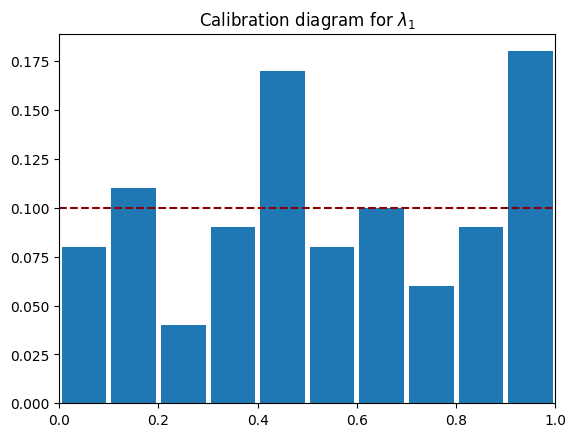
\includegraphics[width=.19\textwidth]{images/sbi_sir/run_2/degen calib lambda1.png}
    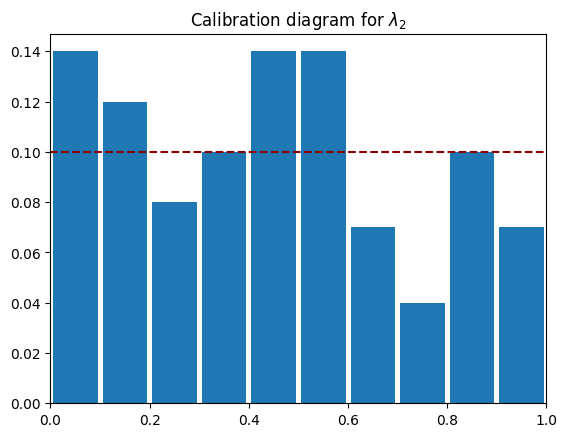
\includegraphics[width=.19\textwidth]{images/sbi_sir/run_2/degen calib lambda2.png}
    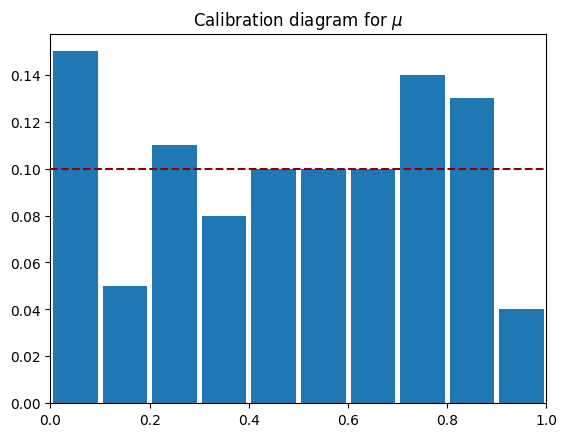
\includegraphics[width=.19\textwidth]{images/sbi_sir/run_2/degen calib mu.png}
    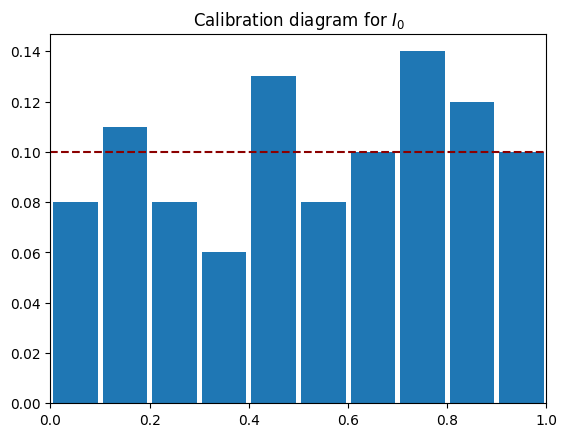
\includegraphics[width=.19\textwidth]{images/sbi_sir/run_2/degen calib I_0.png}
    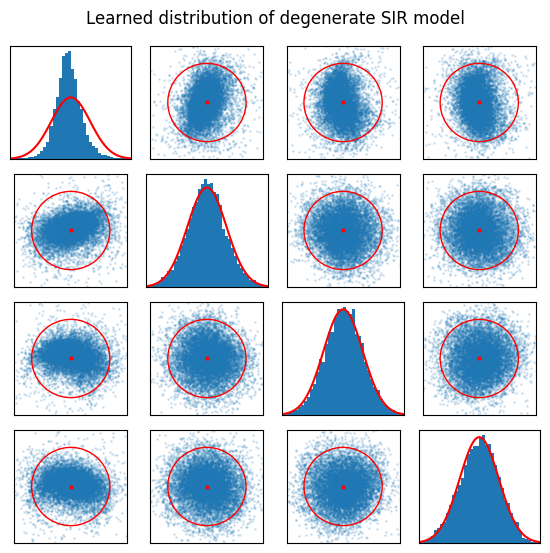
\includegraphics[width=.19\textwidth]{images/sbi_sir/run_2/degen code distribution.png}\\
    \vspace{.5em}
    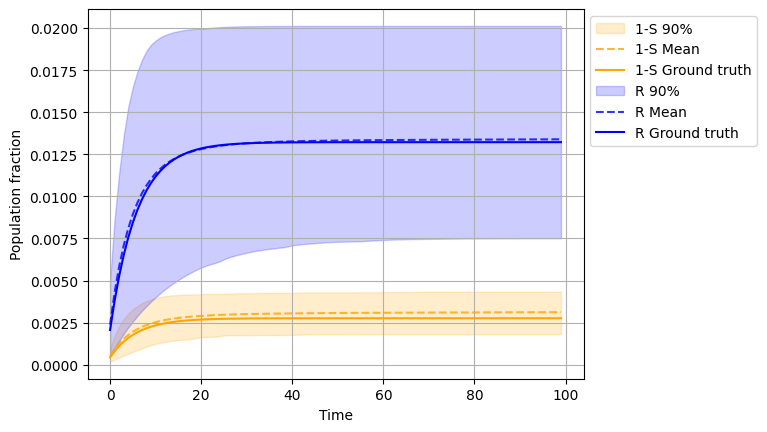
\includegraphics[width=.325\textwidth]{images/sbi_sir/run_2/degen resim 1.png}
    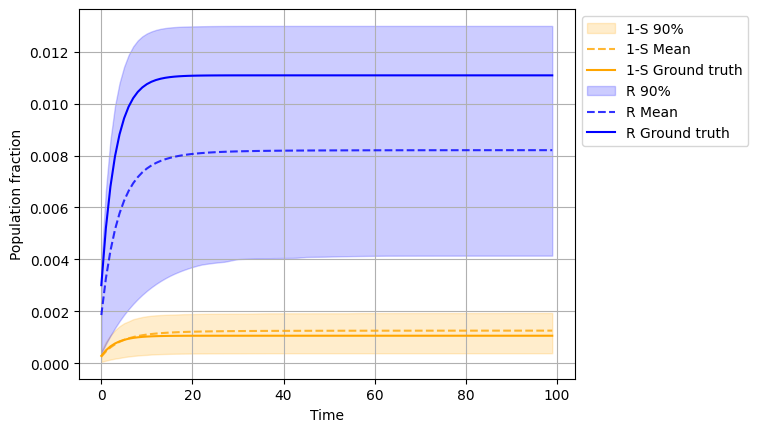
\includegraphics[width=.325\textwidth]{images/sbi_sir/run_2/degen resim 2.png}
    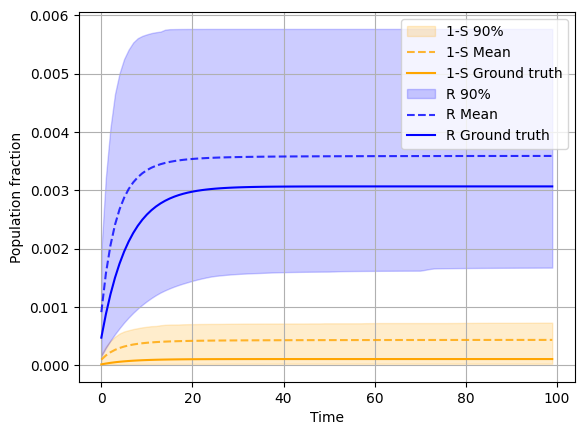
\includegraphics[width=.25\textwidth]{images/sbi_sir/run_2/degen resim 3.png}
    \caption{Calibration diagrams ($\lambda_1$, $\lambda_2$, $\mu$, and $I_0$, respectively), code distribution and three resimulations of degenerate model from the second test.}
\end{subfigure}
\caption{Evaluation data from the second test. }
\label{fig:sir_run_2}
\end{figure}

\begin{itemize}
    \item The code distribution of the basic model looks appalling while that of the degenerate model looks well-behaved except for the first dimension\footnote{Note that the distributions in these plots always have the order $\lambda$, $\mu$, $I_0$ for the basic model and $\lambda_1$, $\lambda_2$, $\mu$, $I_0$ for the degenerate one.}, counter to our expectations. It is also noteworthy that the degenerate model apparently could make better sense of $\lambda_2$ than $\lambda_1$, although this might be down to random chance.
    
    \item The resimulation plots tell a different story: While the ground truth was well within the 90\% confidence interval for both models and all samples, said confidence interval was much narrower for the basic model, insinuating a better understanding of the data.
    
    \item The calibration diagrams all look unpleasant, possibly due to premature training termination. There is no discernible systematic error.
\end{itemize}

In addition to the previously established evaluation data, we also looked at the distribution of sampled parameters for a fixed condition (i.e. the parameters that are used for the resimulation), shown in Figure~\ref{fig:sir_run_2_params}. We were surprised by the spread for the basic model, which is apparently roughly one-dimensional instead of zero-dimensional like we expected, meaning that there is, according to this model, one degree of freedom when fitting parameters to simulation data. In other words, the original ``basic" setup is apparently degenerate. The fact that the resimulation data from this model is so good seems to indicate that this finding indeed stems from the training data itself and not from a poorly trained model. Briefly looking at the sample distribution of the other model, it is clearly higher-dimensional, with the first two dimensions ($\lambda_1$ and $\lambda_2$) forming what looks to be a normal distribution.

\begin{figure}
\centering
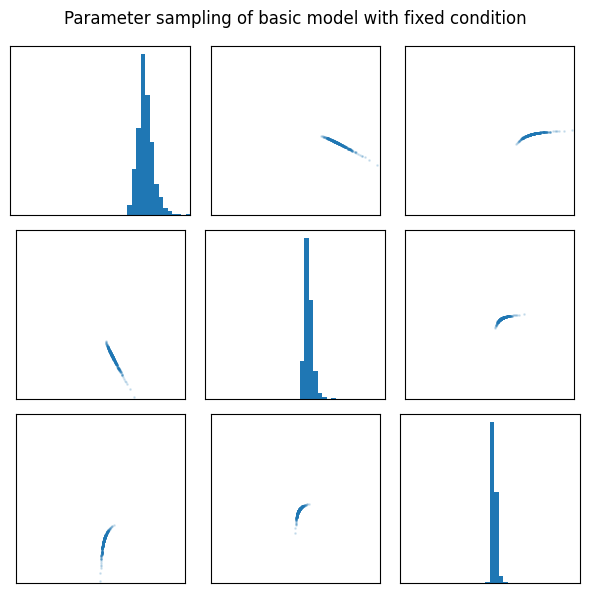
\includegraphics[width=.39\textwidth]{images/sbi_sir/run_2/basic param sampling.png}
\hspace{1em}
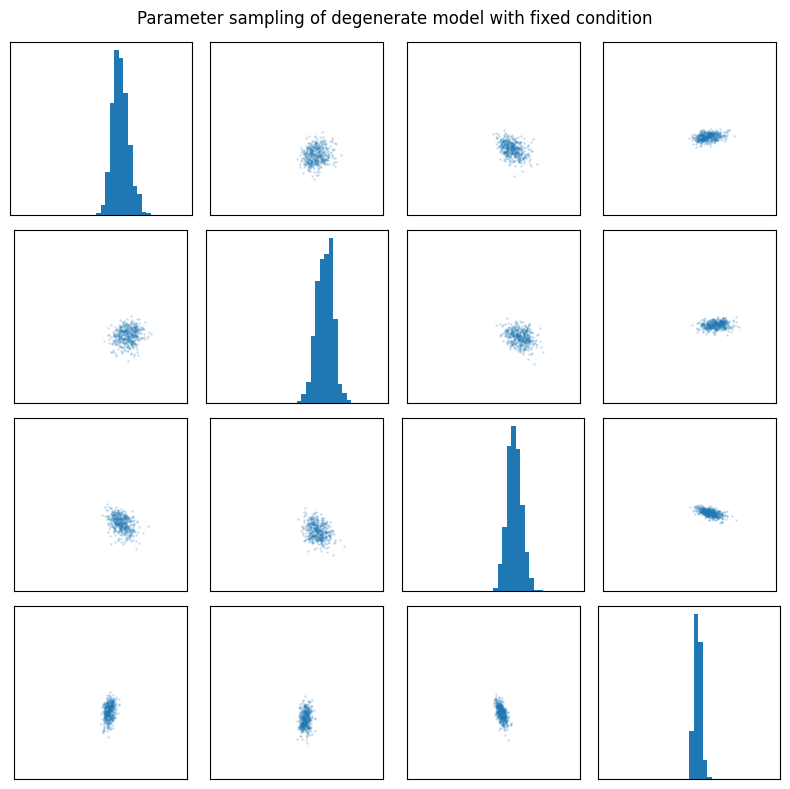
\includegraphics[width=.52\textwidth]{images/sbi_sir/run_2/degen param sampling.png}
\caption{Parameter sample distribution given fixed condition for basic model (left) and degenerate model (right). All subplots are scaled identically, making them easily comparable.}
\label{fig:sir_run_2_params}
\end{figure}

To be candid, we did not know how to proceed from these findings. It is possible that our initial parameter sampling for the model training was chosen badly, resulting in degeneracy of the supposedly unproblematic training set. Even still, we did not know what to make of the model behaviour, i.e. bad code distribution but near perfect resimulation, since this dichotomy indicates that a standard normalizing flow is able to cope with at least mild levels of degeneracy, rendering this whole experiment pointless. We ultimately decided to lay this test series to rest and instead work with much more straight-forward parameter degeneracy.

\asubsubsection{Simple degeneracy}{Jannis Heising}\label{sec:simple_degen}

\textit{The results are taken from the \href{https://github.com/xiaoxiae/GNNFinal2024/blob/main/notebooks/degen_circle.ipynb}{notebooks/degen\_circle.ipynb} notebook.}

As a simple non-trivial example of degeneracy, we chose the dataset to be points on a perfect circle (i.e. without noise) embedded in 2D euclidean space with an arbitrarily chosen radius of 4. This way, the data is two-dimensional, but its intrinsic dimensionality is only One (the only degree of freedom being the angle in polar coordinates). On this dataset, we trained three different models:

\begin{enumerate}
\item A standard normalizing flow with 20 bijective layers (each of course accompanied by an orthonormal layer). This was chosen as a benchmark to compare to.

\item A SurVAE model with two blocks of 10 bijective layers, separated by a bottleneck (referred to as Bottleneck-SurVAE). The bottleneck was achieved by pairing a \texttt{SliceLayer}, which removes one data entry, with an \texttt{Augment-\linebreak Layer}, which appends a random item. In total, the architecture looked as follows:

\begin{minted}{python}
(BijectiveLayer(2, [200, 200]), OrthonormalLayer(2)) x 10,
SliceLayer(2, 1),
AugmentLayer(1, 2),
(BijectiveLayer(2, [200, 200]), OrthonormalLayer(2)) x 10
\end{minted}

This architecture was driven by the desire to reduce the number of data dimensions via a bottleneck, the main obstacle in this simple scenario being that bijective layers need at least two data entries to function. Furthermore, we wanted to use a model that was similar to the chosen NF model in the number of parameters so as to make the results more comparable.

\item A SurVAE model with 20 bijective layers appended by one \texttt{MaxTheLayer} (referred to as Max-SurVAE). The parameters of \texttt{MaxTheLayer} were set to be learnable. The architecture thus is:

\begin{minted}{python}
(BijectiveLayer(2, [200, 200]), OrthonormalLayer(2)) x 20,
MaxTheLayer(2)
\end{minted}

The design choices for this model were basically the same as for the previous one, just using different functionality of the SurVAE toolkit.
\end{enumerate}

Due to time constraints, our only method of evaluating the results was comparing distribution plots.

For the first and only experiment on this dataset, we performed small preliminary tests to find hyperparameters that worked reasonably well for the NF model and then used the same values for the other two models. The idea behind this setup was to compare the models on the NF's ``home territory" so as to, if anything, skew the results in the baseline's favor. The results are shown in Figure~\ref{fig:circle_results}.

\begin{figure}
\centering
\begin{subfigure}{\textwidth}
    \centering
    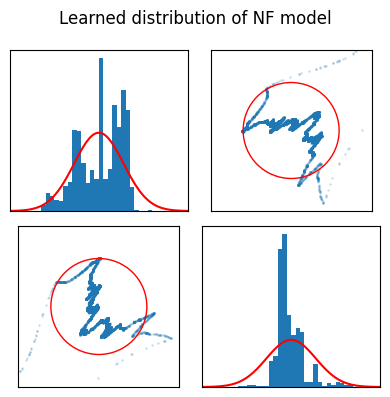
\includegraphics[height=.39\textwidth]{images/degen_circle/nf_code_distribution.png}
    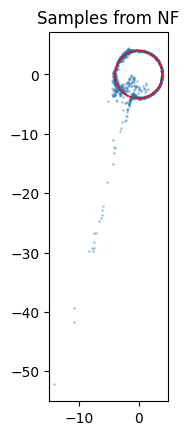
\includegraphics[height=.39\textwidth]{images/degen_circle/nf_sample_full.png}
    \includegraphics[height=.39\textwidth]{images/degen_circle/nf_sample_zoomed.png}
    \caption{Code distribution (left), sample distribution (center), and zoomed-in sample distribution (right) from the NF model.}
\end{subfigure}\\
\vspace{1em}
\begin{subfigure}{\textwidth}
    \centering
    \includegraphics[height=.39\textwidth]{images/degen_circle/sv_bottleneck_code_distribution.png}
    \includegraphics[height=.39\textwidth]{images/degen_circle/sv_bottleneck_sample.png}
    \caption{Code distribution (left) and sample distribution (right) from the Bottleneck-SurVAE model.}
\end{subfigure}\\
\vspace{1em}
\begin{subfigure}{\textwidth}
    \centering
    \includegraphics[height=.39\textwidth]{images/degen_circle/sv_max_code_distribution.png}
    \includegraphics[height=.39\textwidth]{images/degen_circle/sv_max_sample.png}
    \caption{Code distribution (left) and sample distribution (right) from the Max-SurVAE model.}
\end{subfigure}
\caption{Results from the first and only experiment on the circle data. The sample distributions show the desired output shape in red.}
\label{fig:circle_results}
\end{figure}

Interestingly, the NF model behaves somewhat similarly to that from Section~\ref{sec:sbi} in that the code distribution looks horrendous but the samples look passable (though not stellar). There is a distinct line of outliers in the samples that highlights a complexity in the dataset which, frankly, we did not think about prior to seeing these results: The support of the dataset (a circle in $\mathbb{R}^2$) is not contractible, in particular it cannot be meaningfully transformed into the contractible support of a normal distribution that is all of $\mathbb{R}^2$.

The Bottleneck-SurVAE model performed abhorrently, although its latent distribution looks better than that of the NF.

The Max-SurVAE model undoubtedly produced the best samples. The line of outliers observed in the NF plot appears here as well, but not nearly as pronounced. The latent distribution looks promising, but definitely not perfect. If we had more time, we would certainly perform more tests with this kind of model.

This experiment shows that SurVAE models have the potential to help learn degenerate datasets, although more testing is needed to form a more concrete conclusion.